\documentclass[12pt]{article}

\usepackage[left=1in,right=1in,top=1in,bottom=1in]{geometry}
\usepackage[english]{babel}

\usepackage[colorlinks = true,
linkcolor = black,
urlcolor  = blue,
citecolor = blue,
anchorcolor = blue]{hyperref}
\usepackage[inline] {enumitem}
\usepackage[normalem]{ulem}
\usepackage{soul}
\setul{0.25ex}{}

\usepackage{caption}
\usepackage{subcaption}

\usepackage{tikz}
\usepackage{comment}
\usepackage{multirow}
\usepackage{multicol}
\usepackage{booktabs}
\usepackage{color, amsmath}
\usepackage{mathtools}
\usepackage{setspace}
\usepackage{lastpage}
\usepackage{fancyhdr}
\usepackage{float}
\usepackage{graphicx}
\usepackage{amsmath}
\usepackage{amsfonts}
\usepackage{amssymb}


\setlength{\parskip}{1em}
\setlength\parindent{0pt}
\pagestyle{fancy}
\fancyhf{}
\chead{TransportBench Dataset}
\cfoot{Page \thepage\ of \pageref{LastPage}}
\graphicspath{{figures}}

\newcommand{\tp}{T}
\newcommand{\bmtx}{\begin{bmatrix}}
\newcommand{\emtx}{\end{bmatrix}}
\newcommand{\bsmtx}{\left[ \begin{smallmatrix}} 
\newcommand{\esmtx}{\end{smallmatrix} \right]} 
\newcommand{\bmatarray}[1]{\left[\begin{array}{#1}}
\newcommand{\ematarray}{\end{array}\right]} 

\newcommand{\bmat}[1]{\begin{bmatrix} #1 \end{bmatrix}}
\newcommand{\pmat}[1]{\begin{pmatrix} #1 \end{pmatrix}}

\usepackage{graphicx} % For \resizebox
\usepackage{amssymb}  % For \times and \checkmark
\usepackage{tikz}

% Define a new command for the combined checkmark and times symbol
\newcommand{\halfcheck}{
\tikz[scale=0.6,baseline=-0.5ex]{
    % Draw checkmark
    \draw[line width=0.8pt] (0,0.2) -- (0.2,0) -- (0.6,0.4);
    % Draw times
    \draw[line width=0.8pt] (0.2,0.4) -- (0.6,0);

}%
}

% Custom command to include section number in subsection*
\newcommand{\customsubsection}[1]{
  \subsection*{Problem \thesection.#1}
}



\begin{document}


Listed below are the comprehensive topics from which we have extracted questions, covering various aspects of transportation system engineering, to compile our dataset.

\textbf{Table of Contents:}
\begin{enumerate}
\item Facts
\item Transportation economics 
\item Driver Characteristics
\item Vehicle motion
\item Geometry design
\item Traffic flow$\backslash$control 
\item Transportation planning
\item Utility and mode split
\item Transportation networks 
\item Transit systems 
\end{enumerate}

For each problem, we first provide the problem statement and then the solution.



\newpage


\section{Facts}
Problems 1-14 are True/False and 15-22 are open ended questions.

\customsubsection{1}
FTA represents Federal Transportation Administration, a federal government agency within the US Department of Transportation. True or False? 


\textbf{\textcolor{red}{Solution :}} \\
False (Federal Transit Administration)  

\newpage


\customsubsection{2}
In recent years, approximately 20\% of GDP is accounted for by expenses related to the transportation sector, and transportation covered nearly 10\% of household consumption expenditures. True or False? 


\textbf{\textcolor{red}{Solution :}} \\
False (9.0\% of GDP in 2022; 16.8\% household consumption in 2022)

\newpage

\customsubsection{3}
In Year 2000, the U.S. transportation industry shares more than 50\% of the nation’s energy consumption. True or False? 


\textbf{\textcolor{red}{Solution :}} \\
False (27.4\%.)

\newpage

\customsubsection{4}
In year 2001, the U.S. transportation industry consumes more energy than the U.S. production industry. True or False? 


\textbf{\textcolor{red}{Solution :}} \\
False (Transportation: 27.3\%; Industrial: 33.7\% ) 

\newpage



\customsubsection{5}
FHWA, FAA, AASHTO, IDOT, and AAR all stand for government transportation agencies. True or False? 


\textbf{\textcolor{red}{Solution :}} \\
False. The Association of American Railroads (AAR) is a (private) trade association.

\newpage

\customsubsection{6}
In Year 2003, only about four thousand fatal transportation accidents in total occurred in the United States. True or False?


\textbf{\textcolor{red}{Solution :}} \\
False (42,884 fatal motor vehicle fatalities)

\newpage

\customsubsection{7}
Before the Interstate highway system was constructed, it took Lt. Col. Eisenhower’s convoy more than 60 days to travel from Washington DC to S.F in 1919. True or False.


\textbf{\textcolor{red}{Solution :}} \\
True (62 days)
\newpage

\customsubsection{8}
The transportation industry is highly deregulated, and government influence has become negligible. True or False? Explain your answer.


\textbf{\textcolor{red}{Solution :}} \\
False. The transportation industry is governed by many federal and local authorities. In aviation, for example, the FAA tightly controls and monitors the US airspace. Other governmental agencies which oversee the industry through laws and policies include the FMCSA, NHTSA, EPA, STB, FMC, and the FTA. State and local DOTs also regulate and/or operate the industry.
\newpage


\customsubsection{9}
Someone who never travels can benefit from the improvement of a transportation system. True or False? Explain your answer. 


\textbf{\textcolor{red}{Solution :}} \\
True. Improvement of transportation systems (e.g. by making them more efficient, resilient, and/or more sustainable) can benefit non-users by reducing cost/price of products and services. There are also indirect benefits to non-users from energy/environmental enhancements.
\newpage

\customsubsection{10}
Public carriers are owned and operated by public agencies to provide transportation service to the society. True or False? Explain your answer. 


\textbf{\textcolor{red}{Solution :}} \\
False. Public carriers provide service to the general public. They can be owned by public agencies or private companies.

\newpage

\customsubsection{11}
Public carriers (i.e., those serving the public), by definition, try to provide quality transportation service and maximize social welfare. True or False? Explain your answer. 


\textbf{\textcolor{red}{Solution :}} \\
False (public carriers include firms that are for-profit and are not necessarily concerned with maximizing social welfare)
\newpage


\customsubsection{12}
Private carriers are generally owned and operated to serve own needs.  True or False? Explain your answer. 


\textbf{\textcolor{red}{Solution :}} \\
True. Private carriers are generally for-profit entities that are not obliged to serve the entire public. This is in contrast with public carriers who are obliged to serve the public.
\newpage

\customsubsection{13}
Transportation systems generally include two components: moving parts (e.g., vehicles) and fixed parts (e.g., physical guideway and abstract network). True or False? Explain your answer. 


\textbf{\textcolor{red}{Solution :}} \\
False. They should also include operating rules and control mechanisms (e.g. right of way).
% No. (They should also include operating rules and control mechanisms (e.g. right of way).

\newpage

\customsubsection{14}
Railroad provides an energy-efficient and cheap mode for freight transportation. True or False?


\textbf{\textcolor{red}{Solution :}} \\
True. Transporting freight by rail is often cheaper and much more energy efficient than by truck or air.
\newpage


\customsubsection{15}
List five critical issues in transportation engineering.


\textbf{\textcolor{red}{Solution :}} 
Below are some issues:
\begin{enumerate}
    \item Improving efficiency (reducing congestion)
    \item Improving safety
    \item Responding to climate change
    \item Promoting equity and inclusion
    \item Building a strong economy
    \item Advancing public health
    \item Enhancing resiliency
    \item Workforce development
\end{enumerate}

\noindent Source: Critical Issues in Transportation for 2024 and Beyond (2024) and earlier versions.

\newpage

\customsubsection{16}
List five transportation modes in transportation engineering. 


\textbf{\textcolor{red}{Solution :}} 
\begin{enumerate}
    \item [a.] Railway transport
    \item [b.] Roadway transport
    \item [c.] Air transport
    \item [d.] Pipeline transport
    \item [e.] Maritime/waterway transport
\end{enumerate}
\newpage



\customsubsection{17}
Briefly describe the components that constitute a typical transportation system, and give one example for each.


\textbf{\textcolor{red}{Solution :}} 
\begin{itemize}
    \item Moving parts. The parts of a transportation system that move people/goods, e.g. cars, trains, aircraft;
    \item  Physical infrastructure. The parts of a transportation system that act as guideways for the moving parts, e.g. roadway, railway, waterway;
    \item Control infrastructure. The parts of a transportation system that are put in place to manage or control the movement of the moving parts for reasons of safety, efficiency, e.g. right of way priorities.
\end{itemize}
\newpage


\customsubsection{18}
Briefly describe how government is involved in the transportation industry (e.g., private and public carriers). 


\textbf{\textcolor{red}{Solution :}} 
Below are some bullet points:
\begin{itemize}
    \item The government enacts laws and policies that control the physical usage of transportation infrastructure by the public, and public and private carriers
\item The government sets goals for the transportation industry (e.g. improve public health, mitigate environmental damage)
\item The government invests in planning, construction, and operations of transportation infrastructure
\item The government invests in transportation research and development

\end{itemize}
\newpage


\customsubsection{19}
Briefly describe the possible positive and negative effects of two emerging technologies in the transportation industry.

\textbf{\textcolor{red}{Solution :}} 
Below are just two examples.
\begin{itemize}
    \item [1.] \textbf{Autonomous and connected vehicles} As autonomous and connected vehicle technology improves, the number of vehicle crashes will likely be reduced, and traffic flow efficiency can improve through the synchronization of connected autonomous vehicles. There may be further impacts on land use, urban form, and life style. However, autonomous vehicles might increase the risk of cyber-security, and disrupt the job security of drivers (e.g. taxi/truck/bus drivers).
    \item[2.] \textbf{Electric vehicles} Electric vehicles have the potential to significantly reduce carbon emissions from the transportation sector, and increase sustainability, but the batteries are resource-intensive and their extra weight can increase the amount of non-tailpipe emissions (e.g. brake dust). EV also impose higher charging time and driver anxiety.
\end{itemize}

\newpage


\customsubsection{20}
Briefly summarize how improved transportation systems can benefit the society as a whole. 


\textbf{\textcolor{red}{Solution :}} \\
Society benefits from improved transportation systems because investing in well-planned and well-designed transportation systems improves the quality of life for its users by many metrics. From an economic standpoint, improving transportation systems can increase the time/space utility of goods, giving rise to specialization and economies of scale. In terms of health, improving transportation systems (e.g. by building more bike lanes and public transit) can decrease negative externalities such as air/noise pollution. 
\newpage


\customsubsection{21}
Describe the roles of the transportation “non-users” (i.e., government, professionals, and general public) in the U.S. transportation industry (regarding public and private carriers). 


\textbf{\textcolor{red}{Solution :}} \\
\textbf{Government}
on public carriers:
\begin{itemize}
    \item [a.] Own/operate vehicles and infrastructure
    \item[b.] Subsidize transit systems
    \item[c.] Regulate, e.g. controlling air pollution
    \item[d.] Expedite/facilitate transportation research through grants 
\end{itemize}

On private carriers:
\begin{itemize}
    \item [a.] Regulate private carriers; e.g., via licensing, axle load limits, safety regulations, and taxes.
\end{itemize}

\textbf{Professionals}
The primary goal of professionals in the transportation industry is to improve operations and efficiency through research, planning, policy-making, and educating the public. 

\textbf{Public} As "non-users", the public is still affected by the transportation industry through externalities such as noise/air pollution and taxation. The public also indirectly influences transportation policies.

\newpage
   


\customsubsection{22}
Describe both positive and negative roles of transportation in the economy. 


\textbf{\textcolor{red}{Solution :}} \\
\textbf{Positive roles:} 

\begin{itemize}
    \item [a.] May improve time/space utility of goods. Note that time utility is the increase of the value of a good from reducing its transportation time (i.e. fast delivery of newspaper, no store sells one week old newspapers). The space utility is related to market expansion, urban sprawl etc. 
    \item [b.] Lead to changes in urban form, land use, e.g., by allowing people to work at jobs farther away. 
\end{itemize}

\textbf{Negative roles:} 
\begin{itemize}
    \item [a.] Consumes user time, money, and other public resources 
    \item [b.] The physical infrastructure and vehicles can be harmful to safety (via crashes) and the environment (via emissions).
\end{itemize}

\newpage




\section{Transportation Economics}
Problems 1-5 are open ended questions.

\customsubsection{1}
Suppose that a metropolitan transit authority needs to provide transit service in a huge linear city of length $L$. The city is homogeneous everywhere. The daily cost of providing transit service in this area is $c_1 x^{-1/2} + c_2 x^2$ (\$/day per station), where $x \ll L$ is the length of the catchment area served by one station along the line and constants $c_1, c_2 > 0$. Determine $n^*$, the optimal number of transit stations, that minimizes total cost incurred to the authority per day. Express it in terms of $L$, $c_1$, $c_2$. 


\textbf{\textcolor{red}{Solution :}} \\
Since there are $n = L/x$ bus stops in the transit system, each with cost $c_1x^{-\frac{1}{2}} + c_2x^2$, we must minimize the function

\[
\min \frac{L}{x}\left( c_1 x^{-\frac{1}{2}} + c_2 x^2 \right)
\]

\[
 = \min L\left( c_1 x^{-\frac{3}{2}} + c_2 x \right)
\]

Minimizing the function by taking the derivative, setting it to 0, and solving for $x$, we have
\[
x^* = \left( \frac{9c_1^2}{4c_2^2} \right)^{\frac{1}{5}}
\]

\[
n^* = L \left( \frac{4c_2^2}{9c_1^2}\right)^\frac{1}{5}
\]


\newpage

\customsubsection{2}
Upon successfully running the “widget” plant at Pittsburgh, you are promoted to manage a newly established overseas manufacturing plant at Arica, the most northern city in Chile. Chile can be considered a linear country that is 2500 miles in length. A competitor has already built a similar plant at Punta Arenas, the most southern city of Chile. Both you and the competitor produce these widgets at a rate of $C = 8.00$ dollars per unit.

Population of potential customers is uniformly distributed with a density of $\delta = 5$ people/mi. The prevailing market price of these widgets is $P = 10.00$ dollars per unit everywhere, and every customer will buy $D = 2$ widgets per person per year. A public carrier is hired by both plants to deliver the widgets to the customers at a cost rate of $f = 10^{-3}$ dollars per widget-mile. To most effectively penetrate into the market, you may choose to offer variable discount prices to certain customers. Your competitor may use the same strategy.

\begin{itemize}
    \item [a.]  While maximizing your own profit, what are your plant’s total revenue, total cost, and total profit?
    \item [b.]  Due to recent technological innovations (confidential from your competitor), you are able to produce these widgets at a rate of $C = 7.00$ dollars per unit next year. Nothing else will change. What will be your total revenue, cost, and profit?
\end{itemize}

\textbf{\textcolor{red}{Solution :}} 

\begin{itemize}
    \item [a.] First, assume there is no competitor. The revenue, \(R\), will be

\[
R = L\delta PD
\]

where \(L\) is the distance to the end point of the serviced length (without the competitor). 
The total cost will be the sum of the transportation cost, \(T\), and manufacturing cost, \(Z\):

\[
Z = L\delta CD
\]

\[
T = f \delta D \int_0^L x \, dx
\]

\[
T = f\delta D \frac{L^2}{2}
\]

The profit for a given \(L\) can then be found by the equation:

\[
\text{Profit} = R - (Z + T)= L\delta PD - L\delta CD -  f\delta D \frac{L^2}{2}
\]

We can maximize the profit by optimizing the above formula over $L$. Specifically, we can take the derivative, setting it to 0, and solving for the optimal \(L^*\):

\[
L^* = \frac{P - C}{f}
\]

which yields a service length for both us and our competitor of 2000 miles. Alternatively, the value of $L^*$ can directly be found by equating the marginal revenue to the marginal cost per widget; i.e., 
$$ P = C+fL.$$

When the competitor is present, by symmetry, the competition will reduce your market to be between 0 and 1250 miles (past \(x = 1250\) our competitor can undercut us). From \(x = 0\) to \(x = 500\) (i.e., the area where our competitor does not serve --- farther than 2000 miles from its plant) we can charge the full price, but for \(x = 500\) to \(x = 1250\), we must offer a discount equal to the profit our competitor earns (in other words, our price must be equal to the competitor's cost). So, our profit will be the sum of profits from the ranges 0-500 and 500-1250:

\[
\text{Profit} = P_{0-500} + P_{500-1250}
\]

\[
\text{Profit}_{0-500} = 500P\delta D - 500C\delta D - f \delta D \frac{500^2}{2}
\]

\[
\text{Profit}_{500-1250} = 750P \delta D - 750C \delta D - f\delta D \int_{500}^{1250} x \, dx - \left( 750P\delta D - 750C\delta D - f\delta D \int_{1250}^{2000} x \, dx \right) 
\]

Simplifying,

\[
\text{Profit}_{500-1250} = -f\delta D \int_{500}^{1250} x \, dx + f\delta D \int_{1250}^{2000} x \, dx
\]

We get \(\text{Profit}_{0-500} = \$8,750.0\), \(\text{Profit}_{500-1250} = \$5,625.0\) for a total profit of \$14,375.0. Our cost, \(Z\), is given by:

\[
Z = 1250C \delta D + f\delta D \frac{1250^2}{2}
\]

which yields \$107,812.5. Our revenue, \(R\), is the sum of the revenue from the two ranges:

\[
R = 500P\delta D + 750P\delta D - \left( 750P\delta D - 750C\delta D - f\delta D \int_{1250}^{2000} x \, dx \right) 
\]

which yields a revenue of \$122,187.5.


    \item [b.] First we must find the point at which both of us would pay the same cost so we set the equations for marginal costs equal to one another. Solving $7 + f x = 8 + f (2500-x)$, we have the market boundary would be at $x=1750$ miles, and the total revenue would be 167,187.5. Total cost would be 137,812.5. The total profit would be 29,375.
\end{itemize}

\newpage

\customsubsection{3}
Upon successfully running the “widget” plant at Pittsburgh, you are promoted to manage a newly established overseas manufacturing plant at Arica, the most northern city in Chile. Chile can be considered a linear country that is 2500 miles in length. Your plant produces the widgets at $C = 8.00$ per unit. A public carrier is hired to deliver the widgets to the customers at a cost rate of $f = 10^{-3}$ dollars per widget-mile. Population of potential customers is uniformly distributed with a density of $\delta = 5$ people/mi. Every customer will need to buy $D = 2$ widgets per person per year if the price is no more than $10$ per widget.

\begin{itemize}
    \item [a.] What are your plant’s total revenue, total cost, and total profit?
    \item [b.] Due to local government’s policy, for any widget sold to the southern part of the country (beyond 1500 miles of length), you are now charged with a local tax of \$0.50. Nothing else changes. What will be your total revenue, cost, and profit?

\end{itemize}

\textbf{\textcolor{red}{Solution :}} 

\begin{itemize}
    \item [a.] First, assume there is no competitor. The revenue, \(R\), will be

\[
R = L\delta PD
\]

where \(L\) is the distance to the end point of the serviced length. The total cost will be the sum of the transportation cost, \(T\), and manufacturing cost, \(Z\):

\[
Z = L\delta CD
\]

\[
T = f \delta D \int_0^L x \, dx
\]

\[
T = fD \delta \frac{L^2}{2}
\]

The profit for a given \(L\) can then be found by the equation:

\[
\text{Profit} = R - Z - T
\]

\[
\text{Profit} = L\delta PD - L\delta CD - f\delta D \frac{L^2}{2}
\]

We can maximize the profit by taking the derivative, setting it to 0, and solving for \(L\):

\[
L^* = \frac{P - C}{f}
\]

which yields a service length of 2000 miles.

The revenue is then \$200,000.00, the total cost is \$180,000.00, and the profit is \$20,000.00.


    \item [b.] This tax will apply to 1000 miles of our current service. For a given \(L\), our new revenue is still 

\[
R = L\delta PD
\]

But our cost is now the sum of the manufacturing cost, \(Z\), the tax, \(F\), and the transportation cost, \(T\):

\[
Z = L\delta CD
\]

\[
T = f\delta D \int_0^L x \, dx
\]

\[
T = f\delta D \frac{L^2}{2}
\]

\[
F = 0.5 (L - 1000)\delta D
\]

Again, taking the derivative of the profit equation, setting it to 0, and solving for \(L\) gives the equation for \(L^*\):

\[
L^* = \frac{P - C - 0.5}{f}
\]

which gives a service length of 1500 miles. Therefore, our revenue is 

\[
R = 1500\delta PD = \$150,000.0
\]

Our cost is 

\[
Z + T + F = 1500\delta CD + f\delta D \frac{1500^2}{2} + 0.5 (1500 - 1000)\delta D = \$133,750.0
\]

So our profit is then \$16,250.0.

\end{itemize}

\newpage



\customsubsection{4}
Upon successfully running the “widget” plant at Pittsburgh, you are promoted to manage a newly established overseas manufacturing plant at Arica, the most northern city in Chile. Chile can be considered a linear country that is 2500 miles in length. You possess advanced production technology to produce the widgets at $C_1 = 6.00$ per unit. A public carrier is hired to deliver the widgets to the customers at a cost rate of $f = 10^{-3}$ dollars per widget-mile.

Population of potential customers is uniformly distributed with a density of $\delta = 5$ people/mi. Every customer will need to buy $D = 2$ widgets per person per year no matter how expensive the widgets are. However, the customers will choose to purchase widgets at the lowest available price. A competitor has already built a plant at Punta Arenas, the southern city of Chile. The competitor produces the widgets at a rate of $C_2 = 8.00$ dollars per unit, and its established rail transportation system allows negligible variable transportation cost.

\begin{itemize}
    \item [a.] While maximizing your own profit, what are your plant’s total revenue, total cost, and total profit?
    \item [b.] The northern part of the country (1000 miles) is mountainous. Due to fuel price increase, the public carrier now charges $1.5f$ per widget-mile for shipping in the mountainous area. Nothing else will change. What will be your total revenue, cost, and profit?
\end{itemize}



\textbf{\textcolor{red}{Solution :}} 
\begin{itemize}
    \item [a.] Let \(P_1\) be the price we sell at, and \(P_2\) be the price our competitor sells at. Were there no competitor, our profit per unit distance at any given distance \(x\) away from Arica would be given by

\[
\text{Profit}_{\text{US}} = P_1 \delta D - C_1 \delta D - f \delta D x
\]

The competitor’s unit profit is independent of the distance, and is given by

\[
\text{Profit}_{\text{COMPETITOR}} = P_2 \delta D - C_2 \delta D
\]

In order for us to maximize our profit, we must set our price at every unit length such that our competitor cannot reduce their price below ours without losing money. Intuitively, we should be able to profit by setting our price below our competitor's lowest possible price up until some point where due to the increasing transportation cost, we can no longer reduce our price. At this point, both us and our competitor will have an equal price since neither can reduce the price without losing money. It will also be at this point where neither can profit, since both of us will have reduced our price such that the profit is 0. We can rewrite the two equations above in terms of the profit instead of price.

\[
P_1 = \frac{\text{Profit}_{\text{US}}}{\delta D} + C_1 + fx
\]

\[
P_2 = \frac{\text{Profit}_{\text{COMPETITOR}}}{\delta D} + C_2
\]

Setting them equal, and setting both profits to 0, we can solve for \(x\):

\[
x = \frac{C_2 - C_1}{f}
\]

Solving for \(x\) yields 2000 miles. Thus, our price (and our competitor's) at 2000 miles from Arica must be set to \$8. Our competitor will set their price to \$8 from \(x = 0\) to \(x = 2000\), so our price will be set to \$8 from \(x = 0\) to \(x = 2000\). Our revenue is then

\[
R = 2000 \cdot \delta \cdot P_1 D = \$160{,}000
\]

Our total cost, \(Z\), is

\[
Z = 2000 \cdot \delta \cdot C_1 D + \delta \cdot f D \int_0^{2000} x \, dx= \$140{,}000
\]

So our profit is \$20{,}000.


    \item [b.] Because the transportation cost for the first 1000 miles increases, our extent of service will decrease. For widgets transported more than 1000 miles, the profit per unit distance is 

\[
\text{Profit}_1 = P_1 \delta D - C_1 \delta D - D \delta f \left(1.5 \times 1000 + x - 1000\right)
\]

Our competitor’s profit is still 

\[
\text{Profit}_2 = P_2 \delta D - C_2 \delta D
\]

Again, rewriting both equations above in terms of the profit instead of price:

\[
P_1 = \frac{\text{Profit}_{\text{US}}}{\delta D} + C_1 + f(x + 500)
\]

\[
P_2 = \frac{\text{Profit}_{\text{COMPETITOR}}}{\delta D} + C_2
\]

Setting the above equal to each other and setting the profits to 0 gives:

\[
x = \frac{C_2 - C_1}{f} - 500
\]

Solving for \(x\) yields 1500 miles. Thus, our price (and our competitor's) at 1500 miles from Arica must be set to \$8. Our competitor will set their price to \$8 from \(x = 0\) to \(x = 1500\), so our price will be set to \$8 from \(x = 0\) to \(x = 1500\). Our revenue is then:

\[
R = 1500\delta P_1 D = \$120{,}000
\]

Our total cost, \(Z\), is 

\[
Z = 1500\delta C_1 D + 1.5 \delta f D \int_0^{1000} x \, dx + 1.5 f \cdot 1000 \cdot 500 \cdot \delta \cdot D + \delta \cdot f D \int_{1000}^{1500} x \, dx
\]

\[
Z = \$111{,}250
\]

So our profit is \$8{,}750.

\end{itemize}
\newpage

\customsubsection{5}
Suppose that you have one widget plant at the center of a sufficiently large country of size $S$ mi$^2$, where population is uniformly distributed with a density of $\delta$ people/mi$^2$. The distances are measured along straight lines (Euclidean metric). The production cost of widgets is $C$ dollars per unit, and the selling price is $P$ per unit, and knows that it can sell $D$ widgets per person per year everywhere in the country. Transportation costs include a fixed portion of $F$ per unit and a variable cost of $f$ dollars per widget-mile. Suppose $P > C + F$.

\begin{enumerate}
    \item[a.] Determine the shape and size of your market (the area your plant will serve). 
    \item[b.] What will be the profit of this one widget plant when $f = 0$?
\end{enumerate}
\textbf{\textcolor{red}{Solution :}} 

\begin{itemize}
    \item [a.] The shape of the market will be circular since it is a Euclidean metric. 
    The boundary of the market will be at the point where the revenue from selling one widget is equal to the cost of producing and transporting it, i.e. $P = C + F + fr$ where $r$ is the radius. Therefore, $r = (P – C – F)/f$. 
    \item[b.] If there is no variable transportation cost, then it will be profitable to serve the entire country under a fixed cost. So the total annual profit is  $M= (P-C-F) \delta S D$. 
\end{itemize}


\newpage
\begin{comment}
    

\customsubsection{6}
A ``widget” manufacturer (e.g., books, kilowatts of electric power, etc…) can produce these widgets at a rate of C = 8.00 dollars per unit. In addition, each production plant costs $C_0 = 2 × 10^6$ dollars per year to operate. The manufacturer has priced these widgets competitively at P = \$10.00 per unit, and knows that it can sell D = 12 widgets per person per year everywhere in the country. Transportation costs will cut into the profit, however. Population is uniformly distributed with a density of $\delta=10 \text{ people/mi}^2$. A public carrier is hired to take the widgets to the customers. It charges f = 10-2 dollars per widget-mile. Distance is measured along a network of N-S and E-W roads so that if the plant is at the origin of coordinates (0, 0) then the distance to reach the customer at point (x, y) is 
\[
z = |x| + |y|.
\]

\begin{enumerate}
    \item Consider a single plant located at the origin and serving the square (defined by $z \leq L$), where L is a parameter with units of miles. Draw a picture and show that the area of the square is $A = 2L^2$. 
    
    \item Write formulae in terms of $A, C_0, C, P, D, \delta$ and $f$ for the plant’s total yearly revenue R and yearly operating cost Z. Prove that the plant’s total transportation cost T is  $ \frac{2^{1/2}}{3} f D \delta A^{3/2}$. Write a formula for the yearly profit, R – (Z+T). 

\item Express now these formulae as a function of A for given values of parameters $C_0, C, P, D, \delta $ and f. Assume the firm covers the continental U.S. ($ 2.5 \times  10^6 mi^2$) with identical plants with square service regions of area A (ignore any gaps at the boundary etc.). Approximately how many plants would be needed and what would be the firm’s yearly profit? Determine (i) the number of plants n that maximizes the firm’s profit, (ii) the corresponding total yearly profit; and (iii) the total transportation cost. 

\item Assume now that the cost of transportation has been eliminated. (Think of a new technology such as the Internet, which has virtually eliminated the transportation cost of books, music, etc). As a result, the firm then operates with only one plant (n = 1) and f = 0. What is the reduction in transportation expenditures? What is the increase in profit for the firm? Are they the same? Why? 

\end{enumerate}
\textbf{\textcolor{red}{Solution :}} \\

\newpage
\customsubsection{7}
This year, you are running an existing ``widget” (e.g., books, kilowatts of electric power, etc…) manufacturing plant at Pittsburgh, which is approximately at the southwest corner of Pennsylvania (PA). Consider PA as a rectangular state with size 200 miles (E-W direction) by 150 miles (N-S direction). Due to state laws, you cannot sell outside of the state. Your manufacturing technology produces these widgets at a rate of C = 4.50 dollars per unit. In addition, each production plant costs $C_0$ = 105 dollars per year to operate. Population of potential customers is uniformly distributed with a density of $\delta = 10 \text{people/mi}2$. All customers are willing to purchase the widgets for at most P = \$6.00 per unit, and every customer will buy D = 10 widgets per person per year. 

Transportation costs will cut into the profit. A public carrier is hired to take the widgets to the customers. It charges $f = 10^{-2}$ dollars per widget-mile. Distance is measured along a network of N-S and E-W roads so that if the plant is at the origin of coordinates (0, 0) then the distance to reach the customer at point (x, y) is 
\[ z = |x| + |y|. \] 

\begin{enumerate}
    \item [a] While maximizing profit, what percentage of the widget market do you occupy this year? What are your plant’s revenue, cost, and profit?  (Hint: The value of $C_0$ definitely influences your cost and profit, but does it affect your market share and revenue?)

You have just learned that, next year, a competitor will build a similar plant at Philadelphia, the southeast corner of PA. The competitor will possess exactly the same manufacturing technology and the same access to the public carrier, etc. Facing this situation, you may choose to offer variable discount prices to certain customers.

\item [b] If you are to maximize your profit under this competition, what percentage of the PA market will you occupy next year? What will be your revenue, cost, and profit? 

The third year, assume that the cost of transportation can be eliminated for you (but not for your competitor), due to your expected acquisition of a ‘secrete’ technology. (e.g., the Internet, which has virtually eliminated the transportation cost of books, music, etc). 

\item [c]	What will be the reduction in your transportation expenditures, from the second to the third year? What will be the increase in your profit? Are they the same? Why?

\end{enumerate}
\textbf{\textcolor{red}{Solution :}} \\

\newpage

\end{comment}



\section{Driver Characteristics}
Problems 1 and 2 are True/False and problems 3-6 are open ended questions.


\customsubsection{1}
Decision sight distance is introduced to engineering practice because stopping sight distance may preclude drivers from performing evasive maneuvers. True or False? Explain your answer. 


\textbf{\textcolor{red}{Solution :}} \\
True. There are situations where drivers have to use a longer reaction/decision time (than what is normally used in computing stopping sight distance) to determine (and conduct) complex evasive maneuvers. 
\newpage

\customsubsection{2}
Generally, stopping sight distance (the distance necessary for the vehicle to come to a full stop) is longer than the decision sight distance. True or False? Explain your answer. 


\textbf{\textcolor{red}{Solution :}} \\
False. Stopping sight distance is the minimum distance required to perceive-interpret-react and brake to a full stop. Decision sight distance is longer because it is the distance the driver needs to perceive and react to more complex situations. In these cases, the driver must digest navigational or hazard information and select an appropriate response (which may not be just braking), the distance traveled is larger than the stopping sight distance.
\newpage

\customsubsection{3}
Briefly state the definition/components of perception-reaction time, their normal design values.


\textbf{\textcolor{red}{Solution :}} \\
Reaction to a stimulus is usually divided into three stages 
\begin{itemize}
    \item \textit{Perception}: \, negligible if a person is warned; about 1 sec if not warned, or 0 sec if the driver is fully alerted. 
    \item  \textit{Interpretation}: \,  depends on complexity; e.g. ~ 1 sec for 3 words 
    \item  \textit{Decision/Reaction}: \, ~ 0.6 – 1.5 sec (use high end for design to be on the safe side).
\end{itemize}

\newpage


\customsubsection{4}
Suppose a student uses a falling ruler to measure reaction time. He noticed a significant difference across trials (i.e., sometimes the ruler fell to the ground, while some other times it did not). What can we infer from that observation? 


\textbf{\textcolor{red}{Solution :}} \\
The reaction time of the student has high variance, possibly because the subject of the test may or may not be fully focused.

\newpage


\customsubsection{5}
Suppose a student uses a falling ruler to measure reaction time. Before the ruler is released, the 0-inch mark is at the same height of the student’s hand. Suppose a student is able to grab the falling ruler at the 10-inch mark. Ignore air resistance. What is the student’s reaction time?

\textbf{\textcolor{red}{Solution :}} \\
First, convert 10 inches to feet $\rightarrow$ 0.83 ft. Using the kinematic equation:

\[
x = x_0 + v_0 t + \frac{1}{2}at^2,
\]

where \(x_0=0, v_0=0, a = 32.2 \, \text{ft/s}^2\). We see that the reaction time was 0.228 seconds.


\newpage

\customsubsection{6}
Suppose a student uses a falling ruler to measure reaction time. Assume the length of the ruler is 10 inch. Before the ruler is released, the 0-inch mark is at the same height of the student’s hand. Suppose a student is not able to grab the falling ruler. Ignore air resistance. What is the minimum value of the student’s reaction time? 


\textbf{\textcolor{red}{Solution :}} \\
First, convert 10 inches to feet $\rightarrow$ 0.83 ft. Using the kinematic equation:

\[
x = x_0 + v_0 t + \frac{1}{2}at^2 > 0.83 \text{ ft},
\]

where \(x_0=0, v_0=0, a = 32.2 \, \text{ft/s}^2\). We see that the reaction time $t >0.228$ seconds.

\newpage


\section{Vehicle Motion}
Problems 1-7 are True/False and 8-11 are open ended questions.


\customsubsection{1}
Due to grade resistance (from gravity), a vehicle will have a higher fuel consumption rate (e.g., per mile) when its tires are flat. True or False? Explain your answer.


\textbf{\textcolor{red}{Solution :}} \\
False (A vehicle will have a higher fuel consumption rate with flat tires, but due to increased rolling resistance; grade resistance will remain the same)
\newpage

\customsubsection{2}
The rolling resistance force (on moving vehicles) is related to the slope/grade of the road. True or False? Explain your answer.


\textbf{\textcolor{red}{Solution :}} \\
False (rolling resistance is primarily due to uneven deformation of the tire and ground surface while the tire rolls on the ground)  
\newpage

\customsubsection{3}
In steady-state (stationary) traffic, density = flow $\times$ speed. True or False? Explain your answer. 


\textbf{\textcolor{red}{Solution :}} \\
False. flow = density $\times$ (space-mean speed) 
\newpage


\customsubsection{4}
At a signalized intersection, everything else being the same, the presence of a downhill grade will increase the likelihood for a driver to be in a dilemma zone. True or False? Explain your answer. 


\textbf{\textcolor{red}{Solution :}} \\
True (Downhill grade increases minimum stopping distances, which tends to widen the dilemma zone.)

\newpage

\customsubsection{5}
If the speed of a vehicle keeps increasing, the aerodynamic resistance will eventually exceed the rolling resistance, because the aerodynamic resistance depends on the velocity of the vehicle while the rolling resistance does not. True or False? Explain your answer. 


\textbf{\textcolor{red}{Solution :}} \\
False (rolling resistance increases with speed; e.g., when speed is zero, there is no rolling resistance.)

\newpage

\customsubsection{6}
The magnitude of aerodynamic resistance force (on moving vehicles) is directly proportional to the vehicle weight, air density, and vehicle speed. True or False? Explain your answer. 


\textbf{\textcolor{red}{Solution :}} \\
False (not directly related to vehicle weight, and proportional to the square of vehicle speed; also dependent on the frontal cross-sectional area size)

\newpage

\customsubsection{7}
Aerodynamic resistance is typically the most important factor affecting train resistance at train speeds below 40 mph. True or False? Explain your answer. 


\textbf{\textcolor{red}{Solution :}} \\
False: The aerodynamic resistance of a train is normally not the most prominent at speeds below 40 mph. Aerodynamic resistance increases with the square of speed, so it becomes the most important factor at higher speeds (e.g., > 65 mph).
\newpage

\customsubsection{8}
Describe basic resistance forces of vehicles, and for each resistance force, list one or more factors that influence its value. 


\textbf{\textcolor{red}{Solution :}} \\
\begin{itemize}
    \item[a.] Rolling resistance
    \begin{itemize}
        \item[i.] Weight or mass
        \item[ii.] Road surface rigidity
        \item[iii.] Tire rigidity/inflation
        \item[iv.] Speed
    \end{itemize}
    \item[b.] Aerodynamic resistance (drag)
    \begin{itemize}
        \item[i.] Speed
        \item[ii.] Air density
        \item[iii.] Frontal cross-sectional area size
        \item[iv.] Shape/size of vehicle (due to turbulence)
    \end{itemize}
    \item[c.] Grade resistance (gravity)
    \begin{itemize}
        \item[i.] Weight or mass
        \item[ii.] Grade of road
    \end{itemize}
\end{itemize}

\newpage

\customsubsection{9}
At time \( t_0 \), a vehicle is with velocity \( v_0 \) at location \( x_0 \). Derive the location profile of a vehicle, \( x(t) \), for \( t \ge t_0 \), when acceleration is constant; i.e., \( a(x, v, t) \equiv a \). Show intermediate steps.


\textbf{\textcolor{red}{Solution :}} \\
The location profile will depend on the initial velocity, initial position, and acceleration constant. To understand how the position will change due to acceleration, it is helpful to plot velocity versus time which we can do because the acceleration is constant.
\begin{figure}[h!]
    \centering
    \includegraphics[width=0.5\linewidth]{img/P4_5.png}
\end{figure}
 
The equation for this line is simply \( v\left(t\right)=v_0+a\left(t-t_0\right) \). Because position is the integral of velocity, we can obtain the location profile by integrating this equation with respect to time
\[
x\left(t\right)=x_0+v_0(t-t_0)+a\left(t-t_0\right)^2/2
\] 

\newpage

\customsubsection{10}
A motorcycle’s skid mark at an accident site is 70 feet long. Collision (onto a parked work-zone construction vehicle) occurred at 20 mile/hour. The road is level. The friction coefficient is 0.35. Help the police to determine the motorcycle’s speed when its brakes were first applied. Ignore air resistance. 


\textbf{\textcolor{red}{Solution :}} \\
First, convert 20 mph to $29.33$ ft/s. We can use the kinematic equation below to find the initial speed:

\[\
u^2 = u_0^2 + 2a\Delta x.
\]

Noting that the deceleration due to braking is $fg$ , we have  
\[
u_0 = \sqrt{u^2 + 2fg \Delta x},
\]

where \(g = 32.2 \, \text{ft/s}^2\), \(f = 0.35\), \(u = 29.33 \, \text{ft/s}\), and \(x = 70 \, \text{ft}\). Solving for \(u_0\), we have that the initial speed is 49.38 ft/s or 33.66 mph.

\newpage


\customsubsection{11}
A motorcycle’s skid mark at an accident site is 80 feet long. Impact occurred at 20 mile/hour. The road is level. The friction coefficient is 0.3. Determine the motorcycle speed when its brakes were first applied. Ignore air resistance.



\textbf{\textcolor{red}{Solution :}} \\
First, convert 20 mph to $ 29.33$ ft/s. We can use the kinematic equation below to find the initial speed:

\[\
u^2 = u_0^2 + 2a\Delta x.
\]

Noting that the deceleration due to braking is $fg$ , we have  
\[
u_0 = \sqrt{u^2 + 2fg \Delta x},
\]

where \(g = 32.2 \, \text{ft/s}^2\), \(f = 0.3\), \(u = 29.33 \, \text{ft/s}\), and \(x = 80 \, \text{ft}\). Solving for \(u_0\), we have that the initial speed is 49.05 ft/s or 33.44 mph.

\newpage




\begin{comment}
    
\customsubsection{12}
The acceleration of a vehicle takes the form

$$a = 3.6 – 0.06 v$$

where v is the vehicle speed in ft/sec. At time 0 the vehicle is traveling at 45 ft/sec.
\begin{enumerate}
    \item [a]	Determine the distance traveled by the vehicle when accelerated to a speed of 55ft/sec.
    \item [b]	Determine the time at which the vehicle attains the speed of 55ft/sec.
    \item [c]	Determine the acceleration of the vehicle after 3 sec.
\end{enumerate}

\textbf{\textcolor{red}{Solution :}} \\

\newpage
\customsubsection{13}
The acceleration of a vehicle takes the form
\[a = 3.5 – 0.05 v\]
where v is the vehicle speed in ft/sec. At time 0 the vehicle is traveling at 40 ft/sec at location x=0.
\begin{enumerate}
    \item [a]	Determine the time at which the vehicle attains the speed of 60ft/sec.
    \item [b]	Determine the distance traveled by the vehicle when accelerated to a speed of 60ft/sec.
    \item [c]	Determine the acceleration of the vehicle after 5 seconds.
\end{enumerate}
\textbf{\textcolor{red}{Solution :}} \\

\newpage
\customsubsection{14}
If the acceleration takes the following form instead:
\[a = 3.5 – 0.05 v – 0.0005 v^2 \]
Numerically simulate and plot the location profile and speed profile as functions of time (for 10 seconds). Start with the same initial condition.
\textbf{\textcolor{red}{Solution :}} \\

\newpage
\customsubsection{15}
The acceleration of a vehicle takes the form
\[ a(t) = 7.2 - 0.06 v – 0.001v^2 \]
where v is the vehicle speed in ft/sec. At time 0 the vehicle is traveling at 45 ft/sec.
\begin{enumerate}
    \item [a] Determine the distance traveled by the vehicle when accelerated to a speed of 55ft/sec.
    \item [b]	Determine the time at which the vehicle attains the speed of 55ft/sec.
    \item [c]	Determine the acceleration of the vehicle after 3 sec.
\end{enumerate}
\textbf{\textcolor{red}{Solution :}} \\

\newpage
\customsubsection{16}
Consider a transport truck that meets Federal maximum width and minimum length requirements, is 13 feet and 6 inches tall.  Suppose that the truck is loaded such that it weighs 85,000 lbs.  The width of the truck is 102.36 inches, and length of the truck is 48 feet.

What propulsive force is needed to travel at 60 mph on a road with a 1\% grade and friction factor of 0.25?  Assume  $\alpha=\frac{\rho}{2}C_DA_f$/mass where air density $\rho$ is 0.074887 $lb_m/ft^3$ and the coefficient of drag $C_D$ is 0.85, and $A_f$ is the frontal cross-sectional area of the vehicle.  Assume the coefficient for rolling resistance $\beta$ is 0.00005 s/ft.  

Assuming the engine power in part (a) is the 90\% of the trucks’ maximum engine power, what would be the maximum speed of the truck as it climbed a 5\% grade hill?

\textbf{\textcolor{red}{Solution :}} \\

\newpage
\customsubsection{17}
The acceleration of a vehicle takes the form
\[ a = 3 – 0.04 v \]
where v is the vehicle speed in ft/sec. At time 0 the vehicle is traveling at 40 ft/sec at location x=0. 
\begin{enumerate}
    \item [a] Determine the time at which the vehicle attains the speed of 60ft/sec.
    \item [b] Determine the distance traveled by the vehicle when accelerated to a speed of 60ft/sec.
    \item [c] Determine the acceleration of the vehicle after 5 seconds.
\end{enumerate}
\textbf{\textcolor{red}{Solution :}} \\

\newpage
\customsubsection{18}
Consider a two-lane highway with stationary traffic. There are two types of vehicles, cars and trucks, each occupying one lane. Cars travel with constant speed $v_c$ and the spacing between any two consecutive cars is $s_c$. Trucks travel with constant speed $v_t$, and the spacing between any two consecutive trucks is $s_t$. 
\begin{enumerate}
    \item [a] Write an expression for the total flow (regarding all vehicles) on this highway.
    \item [b] Write an expression for the space-mean speed on this highway. 
\end{enumerate}
\textbf{\textcolor{red}{Solution :}} \\

\newpage

\end{comment}



\section{Geometry Design}
Problems 1-7 are True/False and problems 8-10 are open ended questions.


\customsubsection{1}
In horizontal curve design, for a given design speed, the larger the road radius, the larger the rate of super-elevation. True or False? Explain your answer. 


\textbf{\textcolor{red}{Solution :}} \\
False. A larger road radius will decrease the centrifugal force experienced by a vehicle as compared to a smaller radius with the same design speed, thus reducing the required super-elevation.
\newpage


\customsubsection{2}
While designing an equal-tangent vertical curve, given initial and final roadway grades and PVI, the parameters in the parabolic function can normally be determined once we find the curve length. True or False? Explain your answer. 


\textbf{\textcolor{red}{Solution :}} \\
True. The equation for an equal-tangent vertical curve is
\[
y = \frac{g_2-g_1}{L}x^2 + g_1x + e_{PVC},
\]
where $g_1$ and $g_2$ are the grades expressed as a decimal,
$L$ is the curve length, and $e_{PVC}$ is the elevation of the PVC. The value of $e_{PVC}$ can be easily found from the elevation of the PVI, as PVC is $L/2$ upstream of the PVI (at $g_1$ grade).
\newpage


\customsubsection{3}
In horizontal curve design, for a given design speed, the larger the road radius, the smaller the rate of super-elevation. True or False? Explain your answer. 


\textbf{\textcolor{red}{Solution :}} \\
True. A larger road radius will decrease the centrifugal force experienced by a vehicle as compared to a smaller radius with the same design speed, thus reducing the required super-elevation.
\newpage


\customsubsection{4}
You are given a railroad curve and a highway curve. You find that the “deflection of angle” of the railroad curve (chord definition) and that of the highway curve (arc definition) have the same numerical value. Hence, the highway curve has a smaller radius. True or False? Explain your answer. 


\textbf{\textcolor{red}{Solution :}} \\
True. The deflection angle is defined as the angle subtended by a chord (for railroads), or by a curve (for highways) 100 ft in length. If the deflection angles are the same, then the highway curve would have a smaller radius because two points connected by a 100 ft curve on a circular arc would necessarily be closer together than two points connected by a 100 ft chord.
\newpage


\customsubsection{5}
Parabolic functions are often used in horizontal curve design to yield a constant curvature (and hence a constant centrifugal force). True or False? Explain your answer. 


\textbf{\textcolor{red}{Solution :}} \\
False. Simple circular arcs are often used in horizontal curve design, which are distinct from parabolic curves which are often used for vertical curves.
\newpage


\customsubsection{6}
Minimum lengths of crest vertical curves as determined by sight distance requirements generally are satisfactory from the standpoint of safety, comfort, and appearance. True or False? Explain your answer. 


\textbf{\textcolor{red}{Solution :}} \\
True. Generally on crest curves the sight distance is long enough to ensure drainage, driver comfort, and aesthetic needs.
%False. Minimum lengths of crest vertical curves as determined by sight distance requirements are often not used in practice. Many states have their own minimum values which account for other design requirements such as safety, comfort, and appearance. For instance, the Illinois Department of Transportation recommends a minimum length of 1000 ft for crest curves on rural highways for aesthetic reasons.
\newpage


\customsubsection{7}
Railroad trains stopping distance generally exceeds sight distance. True or False? Explain your answer. 


\textbf{\textcolor{red}{Solution :}} \\
True. While the stopping distance varies with speed and weight, it is often a mile or more for railroad trains. Often the train operator's sight distance is less than a mile.

\newpage

\customsubsection{8}
Cyclists and pedestrians share a 6 ft wide path (level, with a zero grade) between the roadway and the inside (convex) wall of a long curved tunnel. The radius of the inside tunnel wall is 200 ft. Local cyclists ride in the middle of the path. Pedestrians (who also walk in the middle of the path, and will stop as soon as a cyclist comes into view) will be injured if hit by a cyclist with a speed greater than or equal to 5 mph.

What is the fastest safe speed the cyclists should use that can avoid pedestrian injury? Take the coefficient of braking friction as 0.35 and cyclists’ reaction time as 1 sec.

\textbf{\textcolor{red}{Solution :}} \\
The middle ordinate, \(M_{SSD}\), is the distance between the wall and the center of the path, which is 3 ft. We also know that the radius of the curve that the cyclist travels, $R$, is 203 ft. Using these values, we can calculate the central angle of the curve, $\Delta_{SSD}$, through the equation below:

\[
M_{SSD} = R \left(1 - \cos\left(\frac{\Delta_{SSD}}{2}\right)\right),
\]
and hence
\[
\Delta_{SSD} = 2 \arccos \left(1 - \frac{M_{SSD}}{R}\right) \cdot \frac{180}{\pi} = 19.7^{\circ}.
\]

The distance at which the cyclist first sees the pedestrian can be found using the equation below:

\[
x_{SSD} = \frac{\pi}{180} R \cdot \Delta_{SSD} = 69.86 \, \text{ft}.
\]

\begin{comment}
    
The typical stopping sight distance equation below will not work since the cyclist slows down to 5 mph as opposed to being completely stopped.

\[
x_{SSD} = 1.47ut + \frac{u^2}{30f},
\]

where \(f\) is the braking coefficient. Note that \(u\) is in mph here but we will rewrite this so it is in ft/s.
\end{comment}

Since the cyclist slows down to 5 mph as opposed to coming to a complete stop, we use the following kinematic equation below for the braking distance term of the SSD:

\begin{comment}

\[
u^2 = u_0^2 + 2ax_{\text{braking}}
\]

\[
x_{\text{braking}} = \frac{u^2 - u_0^2}{2a}
\]

Where \(a\) is the braking deceleration (\(a = -fg\)). First, convert the final final impact speed of 5 mph, $u$, to 7.35 ft/s.
\end{comment}

\[
x_{SSD} = u_0 t + \frac{u^2 - u_0^2}{-2fg},
\]
where \(a\) is the braking deceleration (\(a = -fg\)). First, convert the final final impact speed of 5 mph, $u$, to 7.35 ft/s.
Solving for \(u_0\) yields a max speed of 30.64 ft/s or 20.83 mph.

\newpage


\customsubsection{9}
You are determining the speed limit for a mountainous one-way highway segment along the bottom of a cliff. The road segment is level (i.e., zero grade) but contains a horizontal curve. The center line of the lane is 20 ft from the inside (convex) rock wall of the cliff. The radius of the inside wall is 600 ft.

What should the speed limit be (round down to the nearest multiple of 5 mph) to ensure enough stopping sight distance on the curve? Take the coefficient of braking friction as 0.35 and drivers’ reaction time as 1.5 sec.

\textbf{\textcolor{red}{Solution :}} \\
The middle ordinate, \(M_{SSD}\), is the distance between the wall and the center of the highway, which is 20 ft. We also know that the radius of the curve that the vehicle travels, $R$, is 620 ft. Using these values, we can calculate the central angle of the curve, $\Delta_{SSD}$, through the equation below:

\[
M_{SSD} = R \left(1 - \cos\left(\frac{\Delta_{SSD}}{2}\right)\right),
\]

\[
\Delta_{SSD} = 2 \arccos \left(1 - \frac{M_{SSD}}{R}\right) \cdot \frac{180}{\pi} = 29.19^{\circ}.
\]

The stopping sight distance is calculated using the equation below:

\[
x_{SSD} = \frac{\pi}{180} R \cdot \Delta_{SSD} = 315.8 \, \text{ft}.
\]

We can use the stopping sight distance equation to find the speed limit by first solving for \(u\) (mph), the initial speed:

\[
x_{SSD} = 1.47ut + \frac{u^2}{30 \times 0.35},
\]
where $t$ (s) is the driver's reaction time
\[
u = 47.16 \, \text{mph}.
\]

Rounding down to the nearest multiple of 5 gives a speed limit of 45 mph.

\newpage


\customsubsection{10}
You are designing an arterial two-way highway in the hills where the speed limit is 45 miles per hour. At one crest point, you need to design a vertical curve that connects a +5\% grade to a -3\% grade. Let’s assume that the drivers’ eyes are generally 3.5 feet from the ground, while the potential obstructing objects are 2 feet tall. The perception-to-reaction time is 2.5 sec. Can you determine the minimum curve length?


\textbf{\textcolor{red}{Solution :}} \\

The equation for stopping sight distance, in feet, is
\[
SSD = 1.47ut + \frac{u^2}{30\left(\frac{11.2}{32.2} \pm \frac{G}{100}\right)},
\]

where $u$ (mph) is the speed limit, and $t$ (s) is the perception-to-reaction time. We have $G_1 = 5 \%$ and $G_2 = -3 \%$. We use the worst-case SSD, which will occur on the steepest downgrade. In case of a two-way arterial highway, the steepest downgrade is $-5\%$. So the SSD is

\[
SSD = 1.47 \times 45 \times 2.5 + \frac{45^2}{30\left(\frac{11.2}{32.2} - \frac{5}{100}\right)} = 392 \, \text{ft}.
\]

The distance, $S$, at which the driver with eye height $H_1$ first sees the object with height $H_2$ will dictate the minimum curve length, $L_{min}$.

\[
L_{min} = \frac{AS^2}{200(\sqrt{H_1}+\sqrt{H_2})^2},
\]
where $A = |G_2 - G_1|$. Substituting in the heights and setting $S = SSD$ gives
\[
L_{min} = \frac{AS^2}{2158} = 569.7 \, \text{ft}.
\]

Because \(S < L_{min}\), we are done. The minimum curve length is 569.7 ft. 

\newpage




\begin{comment}
    \customsubsection{11}
A sag vertical curve joining grades of -6\% and +2\% must be designed to fit under a very narrow overpass. The lowest point of the overpass is 16 feet over the VPI.
\begin{enumerate}
    \item [a.]	Determine the length of curve that will provide a clearance of 14 ft.

\item [b.]	Calculate the design speed for such a curve (maximum centrifugal acceleration: 0.1g). Ignore the visual obstruction caused by the overpass.

\item  [c.]	Plot a scale profile of the project. Calculate the elevations at all the stations (BVC and EVC). The lowest point of the overpass is at station 100+00 and its elevation is 50.00ft.
\end{enumerate}
\textbf{\textcolor{red}{Solution :}} \\

\newpage

\customsubsection{12}
For the following grades of a parabolic curve at PVC and PVT, identify whether the curve is crest or sag: 

\begin{table}[h!]
\centering
\begin{tabular}{|c|c|c|}
\hline
\textbf{GPVC} & \textbf{GPVT} & \textbf{Answer} \\ \hline
4\% & -2\% &  \\ \hline
3\% & 2\% &  \\ \hline
-1\% & 2\% &  \\ \hline
-1\% & -3\% &  \\ \hline
\end{tabular}
\end{table}
\textbf{\textcolor{red}{Solution :}} \\

\newpage


\customsubsection{13}
Suppose the grades of a parabolic vertical curve at PVC and PVT are $G_1 = 3\%$ and $G_2 = -2\%$. The roadway is to be constructed such that:
\begin{itemize}
    \item the design speed of the highway is 55 mph,
    \item the friction coefficient is 0.3
\end{itemize}

\begin{enumerate}
    \item For the stopping sight distance calculations, we normally use the most negative grade $G_2$. Why?
    \item Compute the stopping sight distance.
\end{enumerate}
\textbf{\textcolor{red}{Solution :}} \\

\newpage


\customsubsection{14}
Suppose the grades of a parabolic vertical curve at PVC and PVT are $G_1 = 3\%$ and $G_2 = -2\%$. The roadway is to be constructed such that:
\begin{itemize}
    \item the design speed of the highway is 55 mph,
    \item the friction coefficient is 0.3
\end{itemize}
To design the vertical curve, make the following assumptions:
\begin{itemize}
    \item perception-reaction time is 2.5 seconds,
    \item drivers’ eyes are 4 ft above the surface of the roadway, and
    \item object height is 3 ft.
\end{itemize}

\begin{enumerate}
    \item Assume $S < L$. What is the resulting minimal length of curve?
    \item Assume $S \geq L$. What is the resulting minimal length of curve?
    \item Which $L$, the one from part iii or that from part iv, should be used in the vertical curve design?
    \item Suppose that the curve starts at 100+00 (ft) at an elevation of 1000 ft. Define the parabolic curve.
    \item What is the elevation at 102+50?
    \item At what station is the maximum elevation?
    \item What is the maximum elevation of the curve?
\end{enumerate}
\textbf{\textcolor{red}{Solution :}} \\

\newpage

\customsubsection{15}
Mike cycles to campus every morning through a curved tunnel. Cyclists and pedestrians share a 3 ft wide path (level, with a zero grade) between the roadway and the inside (convex) wall of this curved tunnel. The radius of the tunnel wall is 100 ft. 

\begin{enumerate}
    \item[a.] If Mike rides in the middle of the path, what is the fastest safe speed that allows him to stop before colliding with an oncoming pedestrian (who also walks in the middle of the path, and will stop as soon as Mike comes into view)? Take the coefficient of braking friction as 0.36 and his reaction time as 1.5 sec.
    \item[b.] If he rides at this speed, what will be his speed at the moment of impact with Mary, who is cycling in the opposite direction at the same speed as Mike (assuming that they both react in one second when they see each other and are unable to pass in the narrow path?)
\end{enumerate}

\textbf{\textcolor{red}{Solution :}} \\

\newpage

\customsubsection{16}
Building is located 15 ft from the centerline of the inside lane of a curved highway with a radius of 500 ft. The road is level. Take the coefficient of braking friction as 0.36 and perception-reaction time as 2.5 sec.

\begin{enumerate}
    \item[a.] Determine the appropriate speed limit (round to the nearest multiple of 5 mph) to ensure stopping sight distance on the curve;
    \item[b.] Determine the rate of super-elevation (assume the coefficient of side friction equals 0.15);
    \item[c.] Suppose the regular speed limit on the straight segment of the highway is 65 mph. How much distance upstream of the point of curve is needed for deceleration? Again, use 2.5 sec perception-reaction time.
\end{enumerate}
\textbf{\textcolor{red}{Solution :}} \\

\newpage


\customsubsection{17}
Design a horizontal curve for a design speed of 70 mph such that the radius, $R$, is 1500 feet and the angle of deflection from P.C. to P.T., $\Delta$, is 60°. Assume that the coefficient of side friction, $f_s$, is 0.11, the friction factor is 0.35, and the curve is to have 0 grade. If the point of intersection (P.I.) of the two tangent lines occurs at station 150+00, find:
\begin{enumerate}
    \item[a.] Tangent Length, $T$
    \item[b.] Station of P.C.
    \item[c.] Curve Length, $C$
    \item[d.] Station of P.T.
    \item[e.] Chord Length, $L$
    \item[f.] Middle Ordinate, $M$
    \item[g.] External Distance, $E$
    \item[h.] Degree of Curvature, $D$
    \item[i.] Superelevation
    \item[j.] What is the minimum clearance distance (from the inside edge of the inside lane) to provide sufficient stopping distance?
\end{enumerate}
\textbf{\textcolor{red}{Solution :}} \\

\newpage

\end{comment}

\section{Traffic Flow/Control}
Problems 1-8 are True/False and problems 9-15 are open ended questions.



\customsubsection{1}
In one signal cycle at an intersection, the effective green time for one approach often equals its actual green phase time plus its yellow phase time. True or False. Explain your answer. 

 
\textbf{\textcolor{red}{Solution :}} \\
True. The effective green time is the amount of time vehicles actually can utilize to clear the intersection, which includes the yellow phase.
\newpage

\customsubsection{2}
Greenshields' model (1930s) conjectures that the average travel speed on a freeway remains relatively constant for all low density (uncongested) traffic.  True or False? Explain your answer. 


\textbf{\textcolor{red}{Solution :}} \\
False (Greenshields conjectured (simply, but incorrectly) that the average speed linearly decreases with density)
\newpage


\customsubsection{3}
In all stationary traffic, time-mean speed equals space-mean speed. True or False? Explain your answer. 


\textbf{\textcolor{red}{Solution :}} \\
False (Note that stationary traffic does not require that all vehicles move at the same speed, hence time and space mean speeds do not need to be equal.)
\newpage



\customsubsection{4}
In all stationary traffic, time-mean speed is larger than or equal to space-mean speed. True or False? Explain your answer.


\textbf{\textcolor{red}{Solution :}} \\
True. Time-mean speed is larger than (or equal to) space-mean speed in stationary traffic because a stationary observer (the observer who measures time-mean speed) will count more (or the same amount of) fast vehicles per unit time than an overhead observer (the observer who measures space-mean speed) will count per unit distance. 
\newpage



\customsubsection{5}
In traffic, density = 1 / headway. True or False? Explain your answer. 


\textbf{\textcolor{red}{Solution :}} \\
False. The inverse of the (average) headway is flow. Density is equal to the inverse of the (average) spacing.
\newpage


\customsubsection{6}
In traffic flow dynamics, we use conservation of vehicles to prove the following fact: ``The line/interface in the time-space diagram separating two traffic states has the same slope as that of the line connecting the corresponding traffic state points on the flow-density fundamental diagram.”  True or False? Explain your answer. 


\textbf{\textcolor{red}{Solution :}} \\
True. Let $\Delta x$ be a small portion of the road where all vehicles are initially in state A. Let $\Delta t$ be the amount of time it takes for all vehicles in $\Delta x$ to end up in state B. Note that in this time, all vehicles entering $\Delta x$ will enter in state A, but will leave $\Delta x$ in state B. The speed of the interface between the two states, $u_{AB}$, is then $\Delta x / \Delta t$. Conservation of vehicles requires that the number of vehicles in $\Delta x$ at time $t_0$ + the number of vehicles entering $\Delta x$ in $\Delta t$ time must equal the number of vehicles leaving $\Delta x$ in $\Delta t$ time + the number of vehicles in $\Delta x$ at time $t + \Delta t$. This situation would be reflected on a time-space diagram as a line/interface between the two traffic states.

\begin{align*}
    \Delta x k_A + \Delta t q_A = \Delta x k_B + \Delta t q_B
\end{align*}

where $k_A$ and $k_B$ are the densities of traffic states $A$ and $B$ respectively, and $q_A$ and $q_B$ are the flows of traffic states $A$ and $B$ respectively. Rearranging terms we have 
\begin{align*}
    u_{AB} = \frac{\Delta x}{\Delta t} = \frac{q_A - q_B}{k_A - k_B}.
\end{align*}

It is easy to see that the above slope is the same slope as the slope of the line connecting two traffic states on the q-k fundamental diagram.
\newpage



\customsubsection{7}
In a cumulative diagram for a traffic network, the horizontal separation between the departure and the arrival curves gives the number of vehicles between the two observers.  True or False? Explain your answer. 


\textbf{\textcolor{red}{Solution :}} \\
False -- cumulative diagram refers to the cumulation of vehicles over time (or sometimes, space). Hence, only the vertical separation should be about the number of vehicles.
\newpage


\customsubsection{8}
Railroad traffic control systems must use electric track circuits to monitor and control train position along a line. True or False? Explain your answer. 


\textbf{\textcolor{red}{Solution :}} \\
False. Block-based control does not need to know exact locations of the train along all points in the line.

\newpage



\customsubsection{9}
Write a formula for the average delay per car for an approach to a traffic signal in terms of arrival flow $\lambda$, saturation flow $\mu$, cycle length $C$, effective red time $R$, and effective green time $G$. State the condition under which it applies.


\textbf{\textcolor{red}{Solution :}} \\

 \begin{figure}[h!]
        \centering
        \includegraphics[width=0.5\linewidth]{img/P6_10.png}
        \caption{Cumulative arrival/departure curve}
        \label{fig:P6_10}
\end{figure}

The average delay is found by dividing the total delay (the shaded area, in units of $\text{vehicles} \cdot \text{time}$) by the total number of vehicles served in a cycle (which should be $\lambda C$, not $n$). By noting that $C = R + G$, the average delay is then
\begin{align*}
    \text{Avg delay} &= \frac{R^2}{2C(1 - \lambda / \mu)}.
\end{align*}
For this equation to apply, the total number of vehicles arriving at the intersection during the cycle must NOT exceed the number of vehicles that can potentially leave the intersection during the effective green time.
\begin{align*}
    \text{Condition: } & \lambda C < \mu (C - R).
\end{align*}
\newpage


\customsubsection{10}
 One approach to a traffic signal has constant arrival flow $\lambda$, saturation flow $\mu$, effective red time $R$, and effective green time $G$. Suppose $G$ is sufficiently large to clear the queue at the end of each cycle. In one cycle, what is the number of vehicles that are actually delayed by the intersection? 

\textbf{\textcolor{red}{Solution :}} \\

 \begin{figure}[h!]
        \centering
        \includegraphics[width=0.5\linewidth]{img/P6_10.png}
        \caption{Cumulative arrival/departure curve}
        \label{fig:P6_10}
\end{figure}

The cumulative arrival/departure curve in Figure \ref{fig:P6_10} demonstrates the delay vehicles experience at the traffic signal. The total vehicle delay experienced (vehicles $\times$ time)  is the shaded area, and the total number of vehicles delayed is $n$. By geometry, we have 
\[
n=\frac{R \lambda\mu}{\mu -\lambda}.
\]
\newpage




\customsubsection{11}
Given Greenshields’ speed-density equation: $v(k) = v_f(1 - k/k_j)$, where $v_f$ is the free flow speed and $k_j$ is the jam density.
    \begin{enumerate}
        \item[a.] Derive the relationship (equation) and sketch the $q – k$ fundamental diagram. Mark important quantities on the diagram (such as $v_f$ and $k_j$).
        \item[b.] What may be the flaw of Greenshields’ theory that makes its fundamental diagram unrealistic?
    \end{enumerate}
\textbf{\textcolor{red}{Solution :}} 
\begin{itemize}
    \item [a.] We have \( q = k v =  k\ v_f(1-\frac{k}{k_j}) \) . This is a parabolic function similar to the following:

    \begin{figure}[h!]
        \centering
        \includegraphics[width=0.5\linewidth]{img/P6_4.png}
        \caption{Flow-density fundamental diagram}
        \label{fig:P6_4}
    \end{figure}
    \item[b.] Speed decreases with density k even when $k \rightarrow 0^+$. This is not realistic as drivers can maintain a near-constant free-flow speed for a range of low density values. 
\end{itemize}

\newpage


\customsubsection{12}
Briefly explain why the slope of the line connecting two traffic condition points in the flow-density fundamental diagram equals the interface shockwave speed between the corresponding traffic conditions in the time-space diagram.\\ 

\textbf{\textcolor{red}{Solution :}} \\
\begin{figure}[h!]
    \centering
    \includegraphics[width=0.75\linewidth]{img/P6_5.png}
    \caption{Flow-density fundamental diagram and time-space diagram}
    \label{fig:P6_5}
\end{figure}

The figure on the left is a time-space diagram. The one on the right is a flow-density fundamental diagram. Each state of traffic (area in the time-space diagram) corresponds to a point in the fundamental diagram.

\begin{itemize}
    \item The line in the time-space diagram separating two states (e.g., A and B) has a defined slope. Geometrical considerations would show that the slope of this line is 
    \[
    u_{AB} = \frac{q_A - q_B}{k_A - k_B},
    \]
    where $q_A$ and $q_B$ are the flows of traffic conditions A and B respectively, and $k_A$ and $k_B$ are the densities of of traffic conditions A and B respectively.
    
    \item Conveniently for us, this is also the slope of the line going through points A and B of the flow-density fundamental diagram, based on simple geometry.
    
%These slopes are the same because both diagrams are derived from solving the conservation equation.
\end{itemize}


\newpage






\customsubsection{13}
Consider a two-lane highway with stationary traffic. There are two types of vehicles, cars and trucks, each occupying one lane. Cars travel with constant speed $v_c$ and the time headway between any two consecutive cars is $h_c$. Trucks travel with constant speed $v_t$, and the headway between any two consecutive trucks is $h_t$. 
\begin{enumerate}
    \item[a.] What is the total density (regarding all vehicles) on this highway?
    \item[b.] What is the space-mean speed?
\end{enumerate}
\textbf{\textcolor{red}{Solution :}} 

\begin{itemize}
    \item [a.] The total density is the sum of the density of each lane

\[
k = k_{car} + k_{truck},
\]

where \(k_{car} = \frac{1}{v_c h_c}\); \(k_{truck} = \frac{1}{v_t h_t}\).

So 

\[
k = \frac{1}{v_c h_c} + \frac{1}{v_t h_t}.
\]

\item  [b.] In 1 space unit, we have \(\frac{1}{v_c h_c}\) many cars and \(\frac{1}{v_t h_t}\) many trucks. We can use these numbers as weights to compute the average speed of all vehicles. This gives the space-mean speed:

\[
\bar{v_s} = \frac{v_c \frac{1}{v_c h_c} + v_t \frac{1}{v_t h_t}}{\frac{1}{v_c h_c} + \frac{1}{v_t h_t}} = \frac{\frac{1}{h_c} + \frac{1}{h_t}}{\frac{1}{v_c h_c} + \frac{1}{v_t h_t}}.
\]
\end{itemize}


\newpage

\customsubsection{14}
Consider a one-lane highway with stationary traffic. There are two types of vehicles, cars and trucks, traveling at the same speed $v$. Every car keeps a time headway $h_c$ from its preceding vehicle (the preceding vehicle could be a truck or a car). Due to safety concerns, every truck will keep a different time headway $h_t$ from the preceding vehicle. 
Suppose that the proportion of trucks in the vehicle stream is $p$. Express the total vehicle flow and total vehicle density on this highway, in terms of the above parameters.


\textbf{\textcolor{red}{Solution :}} \\
The average headway in this one lane, \(\bar{h}\), is \((1-p)h_c+ph_t\). Flow is \(1/\bar{h}\), and hence
\[
\text{Flow } q = \frac{1}{(1-p)h_c + ph_t}.
\]
Since all vehicles on the road have the same speed, the time mean speed and the space mean speed are the same. Density is simply
\[
\text{Density } k = \frac{q}{v}= \frac{1}{v((1-p)h_c + ph_t)}.
\]

\newpage

\customsubsection{15}
Traffic on a two-lane, one-way tunnel obeys a triangular fundamental diagram with the following characteristics: capacity = 4000 veh/hr, free-flow speed = 100 km/hr, jam density = 280 veh/km. A vehicle runs out of gas at 10:00 pm, and parks on the shoulder 1 km into the tunnel, when traffic was freely flowing at 3600 veh/hr. Due to “rubbernecking”, capacity at that incident point reduces to $\mu = 3000$ veh/hr.

\begin{enumerate}
    \item[a.] Draw the fundamental diagram for the tunnel and show all the relevant parameters.
    \item[b.] Determine when the back of the queue will emerge at the mouth (entrance) of the tunnel. Show your work.
    \item[c.] What is the headway downstream of the parked vehicle?
\end{enumerate}
\textbf{\textcolor{red}{Solution :}} 


\begin{figure}[h!]
    \centering
    \begin{subfigure}[b]{0.43\textwidth}
    \centering
    \includegraphics[width=0.98\textwidth]{img/P7_4a.png}
     \caption{}
     \end{subfigure}
     \begin{subfigure}[b]{0.43\textwidth}
     \centering
        \includegraphics[width=\textwidth]{img/P7_4b.png}
     \caption{}
     \end{subfigure}
     \caption{Fundamental diagram}\label{fig:P6_14}
\end{figure}


\begin{enumerate}
    \item [a.] See Fig. \ref{fig:P6_14} (a) for the fundamental diagram.

    \item [b.] We want to find the speed at which the interface between the two traffic states, U (uncongested) and Q (congested), \(u_{UQ}\), moves backwards. Let \(q_U\) be the uncongested flow, and \(q_Q\) be the congested flow, \(k_U\) be the uncongested density and \(\mu\) be the congested density. Then we have

\[
u_{UQ} = \frac{q_U - \mu}{k_U - k_Q}.
\]

And we find that \(u_{UQ} = 9.375 \, \text{km/h}\). Since the mouth of the tunnel is 1 km away, it will take 6.4 minutes for the back of the queue to reach the mouth, or at 10:06 pm.


    \item [c.] Flow downstream is 3000 vehicles per hour. Therefore, headway = 1/3000 hr = 3600/3000 sec = 1.2 sec.

\end{enumerate}



\newpage



\section{Transportation Planning}
Problems 1-4 are True/False and 5-8 are open ended questions.

\customsubsection{1}
In practice, we often use gravity model to determine the number of trips that will be produced in (and attracted to) a certain geographical zone. True or False? Explain your answer. 


\textbf{\textcolor{red}{Solution :}} \\
False. The gravity model determines the number of trips going between zone pairs, but does not determine the total number of trip productions or attractions in each zone. The total productions and attractions for each zone must be known before using the gravity model.
\newpage

\customsubsection{2}
The well-known gravity model originates from an analogy to the gravity force between two planets; it utilizes advanced human behavioral theory with regard to trip destination decisions. True or False? Explain your answer. 


\textbf{\textcolor{red}{Solution :}} \\
False. The basic assumption of the gravity model is that the interaction between two locations decreases with their distance, but increases with the level of activity at each location. The gravity model is not based on human behavioral theory.
\newpage

\customsubsection{3}
In practice, we often use cross-classification models to determine the number of trips from an origin zone to a destination zone. True or False? Explain your answer. 


\textbf{\textcolor{red}{Solution :}} \\
False. The cross-classification model is mainly intended for trip productions, i.e. used in the first step of the demand analysis process. Determining the number of trips from an origin zone to a destination zone is the second step of the demand analysis process.

\newpage

\customsubsection{4}
The cross-classification model often assumes a linear additive structure to simplify complex trip decisions. True or False? Explain your answer. 


\textbf{\textcolor{red}{Solution :}} \\
False. The cross-classification model is data driven and can capture any nonlinear relationships.
\newpage

\customsubsection{5}
In the context of transportation engineering, list the four steps commonly used in demand analysis processes, and briefly describe the inputs/outputs of each step.


\textbf{\textcolor{red}{Solution :}} 
\begin{enumerate}
    \item Trip generation
    \begin{itemize}
        \item Inputs: Land uses, demographics, socioeconomic factors, zone partition 
        \item Outputs: Trip production and attraction for each zone
    \end{itemize}

\item Trip distribution
\begin{itemize}
    \item Inputs: Trip production and attraction for each zone
    \item Outputs: Trip number between each OD zone pair
\end{itemize}

\item Mode choice
\begin{itemize}
    \item Inputs: Trip number between each OD zone pair
    \item Outputs: Proportions of demand for each OD that use each available mode choices 
\end{itemize}

\item Trip assignment/network equilibrium
\begin{itemize}
    \item Inputs: Proportions of demand for each OD that use each available mode choices
    \item Outputs: For each mode and OD pair, equilibrium flow on the available network routes/links
\end{itemize}

\end{enumerate}
\newpage

\customsubsection{6}
Briefly state, in your own words, the strength and weakness of regression model and cross-classification model.


\textbf{\textcolor{red}{Solution :}} \\
\textbf{Regression:} Simple, easy to implement. But the model specification may be unrealistic or lacks theoretical foundation, and parameters may turn out to have “wrong” signs;

\textbf{Cross-classification:} Highly flexible, data driven, and allow complex relationships; but the number of classification types can be large, and thus time-consuming to model.

\newpage

\customsubsection{7}
The gravity model takes a set of given zonal productions and attractions as input. The direct output is a set of trip numbers for all origin/destination zone pairs.  We will find that for each origin zone, the summation of the calculated trip numbers across all destination zones equals the given production number. Is this coincidental? Briefly explain. 


\textbf{\textcolor{red}{Solution :}} \\
It is not coincidental because for each attraction zone j, the model multiplies the production of zone i by the fraction of demand going to zone j. So summing over all j’s will sum to the production of i.

\newpage


\customsubsection{8}
Trip productions and attractions are generally computed separately. At the final stage of trip generation for N zones, what is the one condition that the zonal production numbers ($P_k \,\ k=1,2,\hdots, N$) and zonal attraction numbers ($A_k \,\ k=1,2,\hdots, N$) should theoretically satisfy (but often do not)? What do we do if that condition is not satisfied?


\textbf{\textcolor{red}{Solution :}} \\
The sum of all zonal production numbers should theoretically equal the sum of all zonal attraction numbers. This is from the conservation of trips with the study region. This condition is often violated because independent/different methods are often used to calculate attraction and production. To solve this, some simple scaling ``correction" of attraction numbers can be conducted.

\newpage




\section{Utility and Mode Split}
Problems 1-4 are True/False and problems 5 and 6 are open ended questions.


\customsubsection{1}
In traditional microeconomics theory, a rational human is analytic, well-informed, and willing to sacrifice for others. True or False? Explain your answer. 


\textbf{\textcolor{red}{Solution :}} \\
False – a rational person is greedy/selfish/self-interest-driven, and hence not willing to sacrifice for others.

\newpage

\customsubsection{2}
In traditional economics theory, utility is a cardinal quantification of satisfaction/welfare/happiness. True or False? Explain your answer. 


\textbf{\textcolor{red}{Solution :}} \\
False – it is ordinal. 
\newpage

\customsubsection{3}
In traditional economics theory, a rational person is greedy, analytic, and well-informed. True or False? Explain your answer. 


\textbf{\textcolor{red}{Solution :}} \\
True. A fundamental assumption in traditional economics theory is that people are rational, and that rational people are greedy, analytic, and well-informed. 
\newpage


\customsubsection{4}
According to Wardrop’s Principle, when traffic equilibrium is reached, some routes between an origin/destination pair may have unequal travel costs. True or False? Explain your answer. 


\textbf{\textcolor{red}{Solution :}} \\
True. Those unused routes could have a larger cost.
\newpage



\customsubsection{5}
In the utility theory, what do we mean by “rational human”? Is it realistic? Explain briefly why. 


\textbf{\textcolor{red}{Solution :}} \\
In traditional economics theory, a rational person is greedy, analytic, and well-informed. This assumption is for simplicity of analysis, 
but not fully realistic because in reality people show very complex behaviors (e.g., affected by other factors such as their emotions) and lack access to information or analysis skills.
\newpage



\customsubsection{6}
Given a small island $A$ with $P$ family units, each unit $j$ derives $a_j$ daily in economic benefit by sending a commuter to a city $B$ on the mainland. Island $A$ is connected to city $B$ via both a ferry (with round trip ferry fare $F$) and also a toll bridge (with round trip toll $\delta$ plus other out-of-pocket round trip driving cost $c$). The ferry trip lasts $t_F$ hours (for each way) and the car trip $t_c$ hours (for each way). This commuter values driving time at a rate of $\alpha_j$ \$/hr and riding time at $\beta_j$ \$/hr.

Every family is required to send a commuter to $B$ every day, using one and only one of the two modes.
\begin{enumerate}
    \item[a.] Write the utility functions of a round trip for family unit $j$, for both modes.
    \item[b.] Derive an expression for the demand function for ferry service as a function of $F$; assume that: (i) daily economic benefit $a_j$ and driving time value $\alpha_j$ are the same for every family/commuter ($a_j = a$ and $\alpha_j = \alpha$); and (ii) commuters value ferry riding time $\beta_j$ differently, and for any positive value $\gamma$, the commuters with $\beta_j > \gamma$ form a fraction $e^{-\gamma/4}$ (note that $0 < e^{-\gamma/4} < 1$) of the total population.
    \item[c.] Estimate approximately the percentage change in demand when the fare is reduced 1\%, from \$2 to \$1.98. Try to do this as simple as possible.
\end{enumerate}

\textbf{\textcolor{red}{Solution :}} \\

\begin{enumerate}
    \item [a.]     \begin{align*}
        U_{ferry} &= a_j – 2 t_f \beta_j – F, \,\,
        U_{drive} = a_j – 2 t_c \alpha_j – \delta – c
    \end{align*}

    \item [b.] 
    \begin{align*}
        \text{Pr} \left(U_{ferry}>U_{drive} \right) &= \text{Pr}\left( \beta_j < [2 t_c \alpha_j + \delta + c – F] / (2 t_f)  \right)                          =1 – e^{– \frac{(2 t_c \alpha_j + \delta + c – F) }{8 t_f} }.
    \end{align*} 
    Therefore the demand is given by $P-Pe^{– \frac{(2 t_c \alpha_j + \delta + c – F) }{8 t_f} }$.
    \item[c.] Take the derivative of demand w.r.t. $F$, and let\(\gamma = \frac{2t_c \alpha_j + \delta + c - F}{2t_f}\), we have
    \begin{align*}
        \frac{dD}{dF} &= -\frac{P}{8t_f}e^{\frac{-\gamma}{4}}.
    \end{align*}
    \begin{align*}
        \text{Change in demand} \approx \frac{dD}{dF} \cdot -0.02
    \end{align*}
    
    \begin{align*}
        \text{\% change in demand} &= \frac{\frac{dD}{dF} \cdot -0.02}{P-Pe^{\frac{-\gamma}{4}}} \times 100
    = \frac{0.02\frac{P}{8t_f}e^{\frac{-\gamma}{4}}}{P-Pe^{\frac{-\gamma}{4}}} \times 100
    = \frac{\frac{1}{400t_f}e^{\frac{-\gamma}{4}}}{1-e^{\frac{-\gamma}{4}}} \times 100
    \end{align*}.
    
    
\end{enumerate}



\newpage

\begin{comment}
    

\customsubsection{7}
Given is a narrow island that is 20 km long. Interviews show that $4 \times 10^4$ of the island dwellers would derive a daily economic benefit equal to \$60 by working in the mainland and commuting every day. These people are uniformly distributed along the island. The interviews also show that all these people value travel time equally (\$20.00 per hour of time spent walking, waiting, driving or riding). An 8 km bridge connects the south end of the island to their workplace. The average travel speed by car is 40 km/hr. Parking costs \$10.00 (round trip). Driving costs \$0.5/km. The bridge is financed by means of a toll $\delta$ (\$, round trip).

Derive the demand function for the number of bridge commuting trips as a function of the toll. Plot it. (Hint: Draw a clear picture of the island and write an expression for the utility of a car trip as a function of a household’s distance from the southern tip of the island, $x$. Compare with the utility of not traveling.)
    

\textbf{\textcolor{red}{Solution :}} \\

\newpage


\customsubsection{8}
Given is a narrow island that is 20 km long. Interviews show that $4 \times 10^4$ of the island dwellers would derive a daily economic benefit equal to \$60 by working in the mainland and commuting every day. These people are uniformly distributed along the island. The interviews also show that all these people value travel time equally (\$20.00 per hour of time spent walking, waiting, driving or riding). An 8 km bridge connects the south end of the island to their workplace. The average travel speed by car is 40 km/hr. Parking costs \$10.00 (round trip). Driving costs \$0.5/km. The bridge is financed by means of a toll $\delta$ (\$, round trip).
\begin{enumerate}
    \item[a.] Assume now that $\delta = \$1.00$ and that a rapid transit line covering the island and joining its north end to the workplace is being planned. The fare $F$ (one way) is to be determined. The average speed of transit travel on the island (including stops) would be 25 km/hr. The channel crossing would take 0.25 hrs (one way). Transit users would spend 0.75 hrs (round trip) outside the vehicles waiting and walking. Derive the demand function for daily transit trips as a function of $F$. Plot it. (Hint: Here you will need to compare for different $x$ the utility of transit with the utilities of the automobile and not traveling.)
    \item[b.] If $\delta = F = \$1.00$, determine how many of the transit trips are diverted from the automobile, and how many are induced.
\end{enumerate}

\textbf{\textcolor{red}{Solution :}} \\

\newpage


\customsubsection{9}
A small town on an island has been divided into three traffic zones. Surveys and demographic forecasts were conducted earlier so as to provide data for trip generation and distribution in year 2020. Suppose the outcome of HBW trip generation (i.e., zonal productions and attractions) is given in the following table.
\begin{table}[h!]
    \centering
    \begin{tabular}{|c|c|c|c|c|}
        \hline
        Zone & 1 & 2 & 3 & Total \\
        \hline
        Attractions & 105968 & 123562 & 198456 & 427986 \\
        \hline
        Productions & 230586 & 146462 & 50938 & 427986 \\
        \hline
    \end{tabular}
\end{table}

The survey’s results for the zones’ travel time in minutes were as follows:

\begin{table}[h!]
    \centering
    \begin{tabular}{|c|c|c|c|}
        \hline
        Zone & 1 & 2 & 3 \\
        \hline
        1 & 2 & 10 & 8 \\
        \hline
        2 & 10 & 4 & 5 \\
        \hline
        3 & 8 & 5 & 3 \\
        \hline
    \end{tabular}
\end{table}

The following table shows travel time versus friction factor:

\begin{table}[h!]
    \centering
    \begin{tabular}{|c|c|c|c|c|c|c|c|c|c|c|}
        \hline
        Time (minutes) & 1 & 2 & 3 & 4 & 5 & 6 & 7 & 8 & 9 & 10 \\
        \hline
        Friction factor & 82 & 52 & 50 & 41 & 39 & 26 & 20 & 13 & 11 & 10 \\
        \hline
    \end{tabular}
\end{table}

Now, provide the trip distribution calculations using the gravity model. Adjust the attraction factors for two iterations. Assume $K_{ij} = 1$.

\textbf{\textcolor{red}{Solution :}} \\

\newpage


\customsubsection{10}
A small town on an island has been divided into three traffic zones. Surveys and demographic forecasts were conducted earlier so as to provide data for trip generation and distribution in year 2020. Ignoring the spatial size of the island. It has $P$ family units ($P \gg 1$), each unit $j$ may derive $a_j$ daily in economic benefit by sending a commuter to a factory $C$ on the mainland. All commuters value driving time at a rate of $\alpha$ \$/hr and riding time at $\beta$ \$/hr.

The island is connected by ferry to a port $B$ on the mainland. The round trip ferry fare is $F$. There is a toll road from $B$ to $C$, with round trip toll $\delta$. The out-of-pocket round trip driving cost from $B$ to $C$ to $B$ (excluding toll) is $c$. The ferry trip lasts $t_F$ hours (for each way) and the car trip $t_c$ hours (for each way). 
Alternatively, each commuter may stay home and rest, which yields a positive fixed benefit $R$ for everyone.

\begin{enumerate}
    \item[a.] Write the utility functions for family unit $j$, for both choices (having a round trip and staying home).
    \item[b.] Derive an expression for the demand function for ferry as a function of $F$; assume that people receive different benefit $a_j$ from the trip, and the benefit value is uniformly distributed between 0 and a very large number $G$.
\end{enumerate}
\textbf{\textcolor{red}{Solution :}} \\

\newpage


\end{comment}


\section{Transportation networks}

\customsubsection{1}
Briefly state Wardrop’s Principle. 


\textbf{\textcolor{red}{Solution :}} \\
This principle is the basis of user equilibrium: each user will take the route which minimizes their own time resulting in all USED routes eventually having the same travel time – unused routes may have a higher cost. 
\newpage

\customsubsection{2}
When Nash Equilibrium is reached in a transportation network, no traveler can reduce its travel cost by unilaterally changing its route choice.  Use your own words, briefly explain why the Wardrop’s Principle describes Nash Equilibrium in transportation networks. 


\textbf{\textcolor{red}{Solution :}} 
\begin{itemize}
    \item All used routes (given an origin-destination pair) have equal cost $\rightarrow$ there is no benefit from changing to a used route.
    \item All unused routes (given an origin-destination pair) have higher or equal cost $\rightarrow$ there is no benefit from changing to an unused route.
\end{itemize}
As such, every user is stuck with the current route choice being the best option.


\newpage



\customsubsection{3}
Travel from $O$ to $D$ during the middle of the day can be done by highway (car, drive alone) or transit line. The transit fare and the out-of-pocket driving costs (parking, gas…) are $F$ (\$) and $P$ (\$), respectively. The travel times by transit and car are $T$ (hr) and $C$ (hr), respectively. The latter increases with flow, $x$ (cars/hr), as a known function, $C(x)$. The mid-day travel demand (desired flow) from $O$ to $D$ is steady at $q$ (people/hr). We assume that all people value time equally at a rate of $v$ (\$/hr), and they are rational.
\begin{enumerate}
    \item[a.] Define a network equilibrium problem that will identify the equilibrium modal split: (draw the network and label its links and nodes; identify the O/D flow, link flows, and link cost function for each traveler (in terms of \$).
    \item[b.] Write Wardrop’s equilibrium conditions in this context.
    \item[c.] Suppose 50\% of the travelers stay at home if the generalized cost of their trip is greater than $M$ (\$). Define a revised network (links, nodes, link costs and origin/destination table) that will jointly identify the equilibrium trip choices.
\end{enumerate}
\textbf{\textcolor{red}{Solution :}} \\

\begin{enumerate}
    \item [a.] 

    
    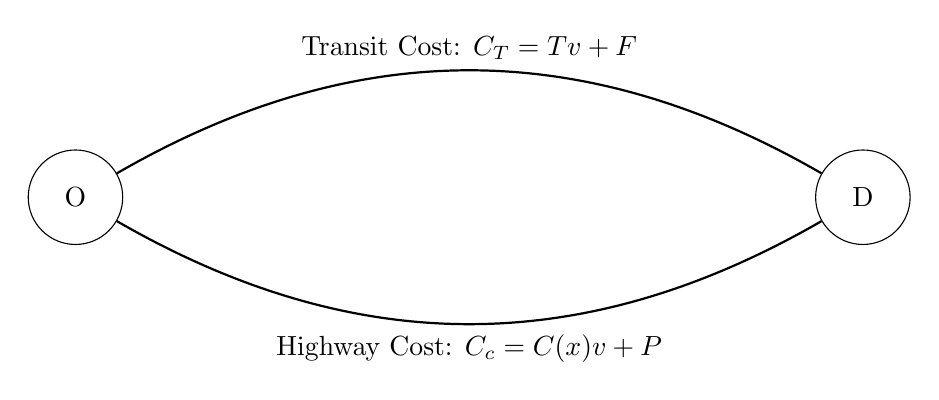
\begin{tikzpicture}
    % Nodes
    \node[circle, draw, minimum size=1.2cm] (O) at (0,0) {O};
    \node[circle, draw, minimum size=1.2cm] (D) at (10,0) {D};
    
   
    \draw[-, thick, bend left] (O) to node[midway, above] {Transit Cost: $C_T = Tv + F$} (D);
    \draw[-, thick, bend right] (O) to node[midway, below] {Highway Cost: $C_c= C(x)v + P$} (D);
\end{tikzpicture}

\item[b.] 

\begin{align*}
    C(x)v + P &= Tv + F \quad \text{if} \quad 0 < x < q \\
    C(0)v + P &> Tv + F \quad \text{if} \quad x = 0 \\
    C(q)v + P &< Tv + F \quad \text{if} \quad x = q
\end{align*}

\item[c.]  
\begin{figure}
    \centering
    \includegraphics[width=0.5\linewidth]{img/Prb9.3.png}
    \caption{Updated network}
    \label{fig:enter-label}
\end{figure}
\end{enumerate}


\newpage



\section{Transit Systems}

\customsubsection{1}
In designing a simple bus corridor using the standards approach, the optimal stop spacing is the same regardless of whether the door-to-door travel time is minimized for the average or worst-case passenger. True or False?


\textbf{\textcolor{red}{Solution :}} \\
False. 

As an example, assume $v_w$ is the walking speed, $s$ is the stop spacing, $l$ is an average travel distance, and $t_d$ is the average vehicle dwell/lost time at each stop.

The worst-case passenger travel time is \( \frac{s}{v_w} + \frac{lt_d}{s}\), and the optimal spacing is
\( s^\ast = \left( l t_dv_w \right)^\frac{1}{2} \),

The average-case passenger travel time is \( \frac{s}{2 v_w} + \frac{lt_d}{s} \), and the optimal spacing \( s^\ast = \left(2 l t_d v_w \right)^\frac{1}{2}
\).

So the optimal spacing varies by a factor of \(\sqrt{2}\).
   
\newpage

\customsubsection{2}
While plotting Vickery diagram for individual transportation shuttle system with $0<e<1\le L<\infty$, it is possible that arrival curve $V(t)$, departure curve $D(t)$, and wish curve $W(t)$ all overlap. True or False? 
    
\textbf{\textcolor{red}{Solution :}} \\
True – when demand is sufficiently low.
\newpage

\customsubsection{3}
Suppose there is a two-point shuttle bus system serving passengers with a non-constant arrival rate. All the buses have large enough capacity. To minimize the average waiting time of passengers, the headway between consecutive dispatched should always be equal. True or False?

\textbf{\textcolor{red}{Solution :}} \\
False. Normally the optimal headway is inversely proportional to the square root of the demand arrival rate.
\newpage

\customsubsection{4}
Consider a city served by a fleet of identical taxis, and all customer trip origins/destinations are uniformly distributed across the city. If the operator decides to add more vehicles into the fleet, the average in-vehicle travel time per passenger is always to decrease. True or False?


\textbf{\textcolor{red}{Solution :}} \\
False. The average in-vehicle travel time will either remain the same or increase (due to more vehicles/traffic) – as the average in-vehicle travel distance remains the same.
\newpage

\customsubsection{5}
For a ride-hailing company serving a service region, additional investment that increases the number of operating taxis will always reduce the average passenger waiting time. True or False?


\textbf{\textcolor{red}{Solution :}} \\
False. Despite a large number of vehicles, the system can be stuck in an inefficient equilibrium known as the ``wild goose chase" in which the average passenger waiting time increases with the number of fleet (as a larger number of vehicles are in the deadheading state).
\newpage

\customsubsection{6}
When we use the standards approach to design a simple bus corridor, the optimal stop spacing would be doubled if the door-to-door travel time in the design standards is based on an average passenger instead of the worst-case passenger (while everything else remain the same). True or False?


\textbf{\textcolor{red}{Solution :}} \\
False. The optimal stop spacing would increase by a factor of $\sqrt{2}$.
\newpage

\customsubsection{7}
You are going to design bus networks for two cities of similar size and shape, under the same investment budget. The ideal type of network (Loop, Hub-and-spoke or Grid) for both cities must be similar. True or False?


\textbf{\textcolor{red}{Solution :}} \\
False. There are other factors which might affect the ideal network such as demand density, population's value of time.
\newpage

\customsubsection{8}
Suppose there is a shuttle bus system serving passengers with a constant arrival rate. All the buses have large enough capacity. If we want to minimize the average waiting time of the passengers, the headway between consecutive dispatches should always be equal. True or False?


\textbf{\textcolor{red}{Solution :}} \\
True. Total waiting time increases with the square of the headway, so the total waiting time for two unequal headways will be larger than the total waiting time if the two headways instead both take the average value.
\newpage

\customsubsection{9}
In a dial-a-ride system, if each vehicle alternates between pickups and deliveries while have a target occupancy level of 7 passengers, then on average each passenger experiences 7 pickup-and-delivery cycles until his/her own drop-off. True or False?


\textbf{\textcolor{red}{Solution :}} \\
True. Expectation of a geometric distribution, with the probability of success (drop-off) being 1/7.
\newpage

\customsubsection{10}
A smooth differentiable univariate function $f(x)$ may not reach a local optimum at point $x_0$ even if the first order condition holds at $x_0$, i.e. $f' (x_0) =0$. True or False?


\textbf{\textcolor{red}{Solution :}} \\
True. The point may be a saddle point.
\newpage

\customsubsection{11}
Sufficiently large buses (infinite capacity) are used to provide shuttle service, and we always optimize dispatch frequency based on the demand. As the temporal demand distribution becomes more uneven (i.e., heterogeneous over time, but no change in total number of passengers), the total (agency + user) cost increases. True or False?


\textbf{\textcolor{red}{Solution :}} \\
False. With a fixed total demand, time-dependent demand variations actually reduces the total cost, because such demand is easier to aggregate into shared vehicles.
\newpage

\customsubsection{12}
The agency is trying to decide whether to design a hub-and-spoke network or a grid network to serve a city with uniformly distributed passenger O/D demand. As agency investment (total service route length per unit area) approaches infinity, these two types of networks eventually yield the same expected door-to-door passenger travel time. True or False?


\textbf{\textcolor{red}{Solution :}} \\
False. A grid network will yield a lower asymptotic door-to-door passenger travel time.
\newpage


\customsubsection{13}
If the daily cost for a transportation system to serve a steady demand of rate $\lambda$ [passengers/day] is $ Z= C\lambda^{1.05}$ [\$/day], where $C$ is a constant, then we say this system has ``economies of scale". True or False?


\textbf{\textcolor{red}{Solution :}} \\
False. The exponent of $\lambda$ would need to be less than 1, so that increase in $\lambda$ would lead to decrease in cost per unit demand, $Z/\lambda$.

\newpage

\customsubsection{14}
For all types of transit networks, the average passenger travel time decreases as the total route length per unit area increases. True or False?


\textbf{\textcolor{red}{Solution :}} \\
False. For a loop type of network, the longer the route, possibly there could be more passenger in-vehicle riding time due to circuitous routes.


\newpage

\customsubsection{15}
Under the “Vickrey equilibrium”, the driver who last arrives at the bottleneck always experiences the smallest in-vehicle delay time (at the bottleneck). True or False?


\textbf{\textcolor{red}{Solution :}} \\
%True. 
False. For example, in case the lateness penalty is infinity, and all traveler have the same wished arrival time, then the last driver actually experience the largest in-vehicle delay (but arrives on time).
\newpage


\customsubsection{16}
The worst-case waiting time of passengers traveling in a two-level hierarchical corridor transit system (with common headway $H$), when they have an appointment at the destination and know the schedule, is $3H$. True or False?


\textbf{\textcolor{red}{Solution :}} \\
False. Worst-case waiting at the destination shall be $H$ due to the appointment. The waiting at the transfer is at most $H$ because synchronization is difficult. 

\newpage


\customsubsection{17}
Sufficiently large buses (infinite capacity) are used to provide shuttle services, and we always optimize the dispatch headway based on the demand rate. As the temporal demand distribution becomes more uneven over time (but the total number of passengers remains the same), the total (agency + user) cost increases. True or False?


\textbf{\textcolor{red}{Solution :}} \\
False. With a shuttle system, time-dependent demand actually reduces the total cost.
\newpage


\customsubsection{18}
In a congested point-to-point shuttle system with two competing modes (transit and automobile), when we have passengers using both modes, slightly increasing the transit headway intensifies the competition and decreases an automobile user’s cost. True or False?

\textbf{\textcolor{red}{Solution :}} \\
False. Increasing the headway would push more users to drive, and hence increase the automobile driving cost.

\newpage

\customsubsection{19}
If the daily cost for a transportation system to serve a steady demand of rate $\lambda$ [pax/day] is $ Z= C\lambda^{0.5}$ [\$/day], where $C$ is a constant, then we say this system has ``economies of scale". True or False?

\textbf{\textcolor{red}{Solution :}} \\
True. As the demand $\lambda$ increases, the average cost per unit demand $ Z/\lambda$ decreases.
\newpage

\customsubsection{20}
Consider designing a realistic corridor system without hierarchy to minimize agency cost, subject to a maximum travel time guarantee $T_0$. As the value of $T_0$ increases, the optimal stop spacing should increase as well. True or False?


\textbf{\textcolor{red}{Solution :}} \\
True. As guarantee $T_0$ (in the right hand side of a constraint) increases, the design problem has a larger feasible region for stop spacing, while the objective function (agency cost) is a decreasing function.
\newpage

\customsubsection{21}
In the context of morning commute, under user equilibrium (Vickrey), the virtual arrival curve and departure curve at the bottleneck will be parallel, both with a slope equal to the bottleneck capacity $\mu$. True or False?

\textbf{\textcolor{red}{Solution :}} \\
False. The slope of the virtual arrival curve may take other values (depending on the earliness and lateness penalty).
\newpage



\customsubsection{22}
In a taxi system, assume taxis are uniformly distributed over space. If the number of idling taxis is doubled, the expected distance from a request location to its closest idle taxi will be approximately half of the distance of the original system. True or False?

\textbf{\textcolor{red}{Solution :}} \\
False. The expected distance will decrease by a factor of $\sqrt{2}$, not 2.


\newpage

\customsubsection{23}
It is found that travel demand fluctuations over time in shuttle bus systems do not have a significant impact on the optimal system costs. This is under the assumption that vehicles are large enough to accommodate all commuters. True or False?

\textbf{\textcolor{red}{Solution :}} \\
True. That is a key assumption for the above description to hold. 
\newpage


\customsubsection{24}
The average-case in-vehicle travel distance for a passenger in a hub-and-spoke system is the same as the one in a grid system. True or False?

\textbf{\textcolor{red}{Solution :}} \\
False. The relative distance ratio is 1 vs. 2/3.
\newpage


\customsubsection{25}
The piece-wise linearity of the virtual arrival curve $V(t)$ in the Vickrey equilibrium is dependent on the assumption that commuters’ generalized cost is a linear function of congestion delay, earliness, and lateness. True or False?

\textbf{\textcolor{red}{Solution :}} \\
True. That is a basic assumption that must hold for the piece-wise linear property.
\newpage

\customsubsection{26}
When designing a non-hierarchical corridor, transit agencies should decrease their headway by  50\% if the passenger value of time increases by 100\%. True or False?

\textbf{\textcolor{red}{Solution :}} \\
False. Headway should decrease by a factor of $\sqrt{2}$, not 2.


\newpage

\customsubsection{27}
One distinct feature of bus transit in the U.S. is the high operating cost per passenger-mile due to low ridership. True or False?

\textbf{\textcolor{red}{Solution :}} \\
True. 
\newpage




\customsubsection{28}
Assume a taxi system operates in a linear city of length L [mile], with passengers’ origins and destinations both uniformly distributed along the line. All vehicles travel at a constant speed v. Passengers arrive according to a Poisson process with rate $\lambda$ [\#/mile-hour], and the dispatcher always immediately assigns a passenger to his/her nearest idle taxi upon arrival. Suppose there are $n$ idle taxis in the system when a passenger arrives, then what is the probability of the passenger waiting more than $a$ units of time (for some $a \ll L/v$ ) until pickup? 

\textbf{\textcolor{red}{Solution :}} \\
The probability of the passenger waiting more than $a$ units of time (for some $a \ll L/v $) until pickup is  \( P(T > a) = (L-2av)^n \).


\newpage


\customsubsection{29}
For a sufficiently long bus corridor with fixed demand, does adding new stops in between the current bus stops guarantee improvement to passengers’ average door-to-door travel speed? 


\textbf{\textcolor{red}{Solution :}} \\
No, adding adding new stops may increase passengers' in-vehicle riding time.



\newpage


\customsubsection{30}
One shuttle ferry with a maximum capacity of 40 passengers travels back and forth between islands A and B, with a round trip time of 0.5 hour, to serve demand in both directions. During the morning peak, travel demand is constant at 2 passengers per minute from A to B, and 1 passenger per minute from B to A. What is the average occupancy of the ferry from A to B and the average occupancy of the ferry from B to A?

\textbf{\textcolor{red}{Solution :}} \\
The average occupancy of the ferry from A to B is 100\% (based on capacity) and from B to A is 75\% (based on demand).


\newpage


\customsubsection{31}
Suppose you encounter a mathematical problem while designing a bus corridor. The expected total cost is a function of spacing $z\left(s\right)=f\left(s\right)+e(s)$, where $f\left(s\right)=a s^2+\frac{b}{s}$ and $e\left(s\right)=0.05\sin^2{(s)}$, where spacing $s>0$, and parameters $a>100$ and $b>50$. Provide a reasonable estimate of the optimal real total cost $z(s^*)$? 


\textbf{\textcolor{red}{Solution :}} \\
Based on Daganzo and Ouyang (2019), one such estimate could be:
\[
z(s^*) \approx 	3\ \sqrt[3]{\frac{1}{4}}\ a^\frac{1}{3}b^\frac{2}{3}+0.05\sin^2{\left(\sqrt[3]{\frac{b}{2a}}\right)}.
\]


\newpage


\customsubsection{32}
In planning a sufficiently long bus corridor with fixed demand, consider the optimal spacing(s) with and without hierarchy. Let $s$ be the optimal spacing without hierarchy, while $s_0$ and $s_1$ be the spacing's of local feeder bus and mainline bus, respectively, within hierarchy. Transfer time/inconvenience is negligible. What is the relation of $s$ to $s_0$ and $s_1$?


\textbf{\textcolor{red}{Solution :}} \\
The relation of $s$ to $s_0$ and $s_1$ is as follows:
\[
s_0 <s \,\ \text{and} \,\ s<s_1.
\]


\newpage



\customsubsection{33}
One shuttle bus (with a capacity of carrying 30 passengers) travels back and forth between a suburban location and the CBD to serve demand in both directions. The travel time each way is 0.15 hour. During the morning, travel demand is constant at 1 passenger per minute from CBD to suburban, and 2 passengers per minute from suburban to CBD. What is the average occupancy of the bus from the CBD to the suburb and what is the flow of passengers served from the CBD to the suburb? 


\textbf{\textcolor{red}{Solution :}} \\
The average occupancy of the bus from the CBD to the suburb is 60\% and the flow of passengers served from the CBD to the suburb is 60 passengers/hour.

\newpage



\customsubsection{34}
The off-ramp of a freeway is congested during 7 – 9 am due to the presence of 2N identical commuters. The wish curve $W(t)$ and the observed departure curve $D(t)$, with respect to this ramp, are given by the following functions:
\begin{align*}
W\left(t\right)&=\frac{N}{2}{(t-7)}^2 \quad t\in[7,\ 9] \\
D\left(t\right)&=N\left(t-7\right) \quad t\in[7,\ 9]
\end{align*}

Under Vickery equilibrium (with $0 < e=0.5 < 1\leq L$), what is the maximum commuter queuing time?


\textbf{\textcolor{red}{Solution :}} This is a case where the lateness penalty must be infinity. The answer is 60 min. \\


\newpage


\customsubsection{35}
A transit agency is trying to minimize the total service miles subject to a given budget. Find the optimal spacing $s$ of the following problem. Use $A=10, \,\ B=40, \,\  C=9,\,\ D=1 \text{ and } M=6$.

\begin{equation*}
\begin{aligned}
\min_{s} \quad & \frac{A}{s} + \frac{B}{s^2}\\
\textrm{s.t.} \quad &  Cs +\frac{D}{s} \leq M\\
  & s \geq 0    \\
\end{aligned}
\end{equation*}


\textbf{\textcolor{red}{Solution :}} 

Note that the first constraint, based on Cauchy Inequality, has to take equality sign. This forces that s=1/3 as the only feasible solution. 
The optimal spacing is $s^*=\frac{1}{3}$.\\ 


\newpage


\customsubsection{36}
A linear city of length 3L is equally bisected by a wide river of length L. Put along the positive direction of an x-axis, its two halves $[0, L]$ and $[2L, 3L]$ are connected through a bridge $[L, 2L]$. Passengers' origins are uniformly distributed (both spatially and temporally) in the residential area ($x\in[0,L]$), and their destinations are uniformly distributed in the CBD area ($x\in[2L,3L]$). An on-call van starts from a depot at the left end of the city ($x=0$) and travels back and forth in the residential area to pick up $n$ customers before heading to the CBD. Upon delivery, the vehicle heads back to the depot to refuel. Ignore the stopping time needed for passenger pick-ups and drop-offs. Suppose that the simple-minded van driver picks up and drops off passengers strictly on the First-Call-First-Served (FCFS) basis, what is the van’s expected travel distance per round trip?


\textbf{\textcolor{red}{Solution :}} 
Track the sequence of travel legs, each with expected length of $L/2$ or $L/3$ or $2L$ depending on the origin/destination pair.
The van’s expected total travel distance per round trip is $\left( \frac{2n+13}{3}\right)L$.\\

\newpage

\customsubsection{37}
A taxi driver has just decided to serve one last passenger before heading home. At the moment, this driver is inside a linear residential area of length W. In this area, there are N randomly distributed passengers. The driver will pick up the nearest one passenger. Find the Pr(the distance to pick-up the nearest one passenger $> a$) for some $a\ll W$? 


\textbf{\textcolor{red}{Solution :}} 
Note independence across passenger locations. Each passenger is at least $a$ distance away from the taxi with a probability of approximately $1- \frac{2a}{W}$. Then,
Pr(the distance to pick-up the nearest one passenger $> a$) \(  \approx \left( 1- \frac{2a}{W}\right)^N\).


\newpage


\customsubsection{38}
A realistic homogeneous transit corridor (e.g., finite speed limit, non-zero stopping penalty, non-zero headway) was optimally designed to minimize agency cost under a single standard. A few years later (now), the passengers’ value of time (e.g., the shadow price of the standard) is about 20\% higher than the original value, while the demand density has increased by 20\% as well. Nothing else changes. If we optimize the system design again under the same standard, by what percentage would the optimal headway approximately change?


\textbf{\textcolor{red}{Solution :}} \\
If we optimize the system design again under the same standards, the optimal headway approximately changes by $\sqrt{2}-1=44$\%.


\newpage


\customsubsection{39}
Considering the “Vickery Equilibrium”, how many and which of the following statements are false?
\begin{enumerate}
    \item The wish curve directly shows the travelers’ wished times to arrive at their final destinations.
    \item The equilibrium condition postulates that no driver is better off by unilaterally changing its arrival time at the bottleneck.
    \item The driver who arrives last at the bottleneck always experiences the smallest in-vehicle delay.
    \item As the wish curve becomes highly non-linear, there may be more than one critical driver (one who arrives at its destination as wished).
    \item If the penalty for lateness and that for earliness are equal, then the slope of the virtual arrival curve for early and late drivers will be equal as well.
\end{enumerate}


\textbf{\textcolor{red}{Solution :}} 

Three of these statements (the 1st, 3rd, and 5th) are false. 

\newpage


\customsubsection{40}
Consider an idealized bi-directional loop line system (i.e., zero headway, zero dwell time at stops, and constant cruising speed), where trip origins/destinations are uniformly distributed in the area. All the stations are placed evenly on square lattices, and their spacing is always chosen to minimize the average walking and riding time. By approximately what percentage would the optimal station spacing change if single-direction service is provided instead?


\textbf{\textcolor{red}{Solution :}} \\
The optimal station spacing change approximately by $\sqrt{2}-1\approx$+40\% if single-direction service is provided instead of bi-directional loop line system.



\newpage

\customsubsection{41}
Suppose the Vickrey equilibrium is always reached around a congested bridge during commuter morning rush hour (say, 7 am to 9 am), suggest a solution that can reduce the maximum length of the queue?


\textbf{\textcolor{red}{Solution :}} \\
A carpool or transit platform adopted by some of the commuters will potentially reduce the maximum length of the queue.

Increase the capacity of the bridge.

Another option is to stagger the wished arrival times of the commuters.


\newpage

\customsubsection{42}
In a grid transit network, for realistic analysis/design, how does the optimal stop spacing change if we optimize the average passenger travel time instead of the worst-case passenger travel time? Quantify the change.


\textbf{\textcolor{red}{Solution :}} \\
The optimal stop spacing change by $\sqrt{2}-1=$+40\% if we optimize the average passenger travel time instead of the worst-case passenger travel time.\\



\newpage

\customsubsection{43}
Suppose we are designing a hybrid transit network with a grid central area and a hub-and-spoke periphery. Assume all buses have the same headway $H$, bus schedules are not synchronized to provide timed transfers, and passengers have appointments at their destination. What is the worst possible total waiting time for the most unlucky passenger?


\textbf{\textcolor{red}{Solution :}} \\
The worst possible total waiting time for the most unlucky passenger will be $4H$ (one each, at the origin station, 2 transfer stations, and the destination station).



\newpage

\customsubsection{44}
Considering the “Vickery Equilibrium”, which of the following statement(s) is (are) false?

\begin{enumerate}
    \item The wish curve is built based on travelers’ wished times to arrive at the bottleneck.
    \item The equilibrium conditions indicate that no driver is better off by unilaterally changing their arrival time at the bottleneck.
    \item The driver who arrives at the bottleneck last may experiences the largest in-vehicle delay time.
    \item As the wish curve becomes highly non-linear, there will always be only one critical driver (one who arrives at its destination as wished)
\end{enumerate}

\textbf{\textcolor{red}{Solution :}} \\
The last (4th) statement is false.


\newpage

\customsubsection{45}
A transit agency is trying to minimize the worst-case travel time while constrained to a given budget. Find the optimal spacing s of the following problem. Use $ \alpha=10,\,\ \beta=40,\,\ \gamma=5 \text{ and } M=5$.

\begin{equation*}
\begin{aligned}
\min_{s} \quad & \frac{\alpha}{s} + \beta s\\
\textrm{s.t.} \quad &  \frac{\gamma}{s} \leq M\\
  & s \geq 0    \\
\end{aligned}
\end{equation*}

\textbf{\textcolor{red}{Solution :}} \\
The convex objective function has a minimum at $s = 0.5$, but that violates the constraint. Therefore, the optimal spacing is at the boundary $s^*=1$. 



\newpage

\customsubsection{46}
%Many cities in the world have CBDs that are surrounded by ring-radial street networks. Assume one such city has a circular CBD with radius, $r > 0$, and that a fraction p of the CBDs area is occupied by skyscrapers with n floors. The average space per employee a, the street spacing s, the street capacity q, and the vehicle occupancy $k =2$. Given this information, estimate the commuter demand [commuters] and the perimeter roadway capacity [commuters/hr]. Then, show how the duration of the rush depends on r, n and p. 

A city with a ring-radial street network has its CBD at the center. The CBD radius is $r$. A fraction p of the CBDs area is occupied by skyscrapers, each with $n$ floors. The average space per employee is $a$, the street spacing is $s$, the street's traffic capacity is $q$, and the vehicle occupancy is $k$. Derive an estimate of the duration of the morning rush hour based on the number of morning commuters, and the roadway capacity around the CBD perimeter. 


\textbf{\textcolor{red}{Solution :}} \\
The total number of commuters can be expressed as \(\frac{pn\pi r^2}{a}\). The maximum number of people able to enter the CBD in one hour is \(\frac{qk2\pi r}{s}\).

If we denote by \(T\) the duration of the rush hour, then the following relationship approximately holds:

\[
\frac{pn\pi r^2}{a} \approx \frac{qk2\pi r}{s} T
\]

Thus,

\[
T = \frac{spnr}{2qka}
\]

i.e. \(T\) is linear with respect to each one of \(p\), \(n\), and \(r\).

\newpage

\customsubsection{47}
%The idea of autonomous (or automated) buses is becoming less and less utopian every day. How do you think such emerging technologies will change the current transit systems in terms of operation, cost and performance? Please discuss briefly. You may consider different scenarios; e.g., (i) a futuristic world where all vehicles are autonomous and connected, and (ii) an intermediate phase when autonomous vehicles and regular vehicles coexist.
How do you think autonomous buses will change the current transit systems in terms of operation, cost and performance? Please consider both a near-term scenario and a far-future scenario.


\textbf{\textcolor{red}{Solution :}} \\
In terms of costs, think about the expenses related to this new technology as compared to drivers’ wages and benefits which initially contribute to 2/3 of the total operating cost.

Also think about how future service hours, fleet management, and parking needs will change as human drivers are no longer needed.


\newpage

\customsubsection{48}
\begin{comment}
Consider an entire two-dimensional plane on which customer demand for some service is homogeneously distributed with density = $\lambda$ [calls/time-area]. Identical service facilities are distributed translationally symmetrically, each serving the calls in an area of equal shape and equal size $A$. These areas tessellate the plane. The cost for providing service to a unit demand is proportional to the Euclidean distance between a customer and its facility with a proportionality factor, $c$ [\$/distance]. Then, 

\begin{enumerate}
    \item use dimensional analysis to show how the average cost of service per unit demand depends on $A$ and $\lambda$.
    \item if the amortized cost of constructing one facility is $f$ [\$/time], derive a closed-form formula for the optimal A.

\end{enumerate}
\end{comment}

In a sufficiently large city, customer demand for service is homogeneous with density = $\lambda$ [1/time-area]. Identical facilities are installed, and each serves an equal area of size $A$. The service delivery cost from a facility to serve a unit demand is proportional to the Euclidean distance by a factor $c$ [\$/distance]. Then, if the amortized installation cost of one facility is $f$ [\$/time], derive a closed-form formula for the optimal $A$.


\textbf{\textcolor{red}{Solution :}} 
\begin{comment}
\begin{enumerate}
    \item  We denote the average service cost per unit demand as \(C \, [\$]\). The dimension matrix can be written as:

\[
\begin{array}{c|cccc}
 & \text{Time} & \text{Distance} & \$ \\
\hline
\lambda &  -1 & -2 & 0 \\
A  & 0 & 2 & 0 \\
c & 0 & -1 & 1 \\
C  & 0 & 0 & 1 \\
\end{array}
\]

This matrix has row dimension $4$ and rank 3, thus the nullity is 1. One such solution is \((0, -\frac{1}{2}, -1, 1)\), giving us the following unitless parameter $\pi$.

\[
\pi = \frac{C}{c\sqrt{A}}, \text{ and hence } \quad C = ac\sqrt{A}.
\]
for some constant $a$, from the Buckingham Pi Theorem.

\item The total cost per call in unit time, which includes the service cost and constructing cost, is

\[
z = ac\sqrt{A} + \frac{f}{\lambda A}, \quad A^\ast = \left( \frac{2f}{\lambda ac} \right)^{\frac{2}{3}}.
\]

\end{enumerate}
\end{comment}

The average delivery distance per unit demand shall be proportional to the square root of the service area size, $\sqrt{A}$, say by a shape factor of $a>0$.
The total cost per facility area per unit time, which includes the service cost and constructing cost, is

\[
z = a c \sqrt{A} + \frac{f}{\lambda A}.
\]

Hence, the optimal $A$ is
\[
\quad A^\ast = \left( \frac{2f}{\lambda ac} \right)^{\frac{2}{3}}.
\]
\newpage

\customsubsection{49}
In the context of Vickrey equilibrium with linear earliness/lateness penalties, can you show that the cumulative virtual arrival curve for a late traveler must be piecewise linear?


\textbf{\textcolor{red}{Solution :}} \\
%Without loss of generality, we only prove linearity for a late person below.
Let \(\mu\) denote the slope of \(D(t)\), and \(w\) the slope of \(V(t)\) for some late person. Assuming we shift \(D(t)\) curve by \(\Delta\), the change in lateness costs is \(\frac{\Delta}{\mu} L \beta\) and the change in delay costs is \(\beta \left( \frac{\Delta}{w} - \frac{\Delta}{\mu} \right)\). At the optimal point, we have 

\[
\lim_{\Delta \rightarrow 0} \frac{\Delta \text{ cost}}{\Delta} = -\frac{1+L}{\mu} \beta + \frac{1}{w} \beta = 0.
\]

Thus 

\[
w = \frac{1}{1+L} \mu,
\]

which completes the proof.

\newpage

\customsubsection{50}
%Consider an idealized non-hierarchical line serving an imaginary campus on the periphery of a circular lake. Passengers' origins and destinations are uniformly distributed along the bus line. This line has zero headway, zero stop time, and an unbounded cruising speed. Please, optimize the design of bus stop spacing assuming that the prevailing passenger travel distance is 4 km, their access speed is 1 m/s, and for comfort reasons, the maximum bus acceleration/deceleration is 2 m/s\(^2\). Now assume you can buy either a transit pass or a bike, but not both, for your travels on this campus. If you know you can ride the bike at an average speed of 5 m/s and your goal is minimizing your on-campus travel time in the long run, will you buy the transit pass or a bike? Why?

%Consider an idealized non-hierarchical line serving an imaginary campus on the periphery of a circular lake. 

Passengers' origins and destinations are uniformly distributed along a circular bus line. Imagine that you have an infinitely large fleet so that the service headway is zero. Also, the bus dwell time at each stop is negligible, and there is no speed limit. You are asked to optimize the bus stop spacing assuming that the prevailing passenger travel distance is 4 km, their access speed is 1 m/s, and for safety concerns, the maximum permitted bus acceleration/deceleration is 2 m/s\(^2\). What is the worst-case passenger door-to-door travel speed under your design?

\textbf{\textcolor{red}{Solution :}} \\

Optimizing for the worst case, we take the total walking time to be \(2 \cdot\frac{s}{2v_w} = \frac{s}{v_w}\) where \(s\) is the stop spacing and \(v_w\) is the walking speed. In the bus, the average passenger will stop at \(l/s\) many bus stops where \(l\) is the prevailing travel distance. Because the bus' cruising speed is unbounded, the fastest option for the bus in between stops is to accelerate from a standstill until it has driven half the distance between two stops, and then decelerate until it reaches a standstill at the next stop. Under this strategy, the travel time in between stops is \(2\sqrt{s/a_0}\), so the total travel time on the bus is \(2ls^{-1/2}a_0^{-1/2}\). The total door-to-door travel time, \(T\), is then

\[
T = \frac{s}{v_w} + 2ls^{-1/2}a_0^{-1/2}
\]
Minimizing this travel time gives an optimal stop spacing of 
\[
s^\ast = \left( \frac{v_w^2 l^2}{a_0} \right)^{1/3} = 200\, \text{m}.
\]

Plugging in the optimal stop spacing into the travel time equation gives an average door-to-door speed of 6.67 m/s. 
\newpage

\customsubsection{51}
%Given is a linear city in the interval \(x \in [-L, L]\). Commuters’ residences are uniformly distributed in the interval \(x \in [-L, 0]\); and their workplaces are also uniformly distributed in the interval \([0, L]\). An arterial corridor runs along the city, on which the city plans to create a transit system that runs one scheduled dispatch in the morning toward the workplaces, and one scheduled return in the afternoon. Passengers’ access stops at speed \(v_w\). The stop spacing is denoted by \(s\). Assume \(L \gg s\). The cruising speed of transit vehicles (not including dwell time at stops) is \(v_t\). The vehicle delay per stop is \(\tau\). The operating cost to the agency (in each service direction) includes two parts: \(c_d\) per unit of bus distance, and \(c_s\) per stop. The agency’s budget is \(B\) [\$/day].

%Formulate a mathematical program that minimizes the users’ average door-to-door travel time in both directions subject to a budget constraint on the agency’s amortized daily expenditures. Find the unconstrained minimum \(s^\ast\); i.e., for \(B = \infty\).

A daily commuter train line serves a linear city in the interval \(x \in [-L, L]\). Commuters’ residences are uniformly distributed in \([-L, 0]\); and their workplaces are uniformly distributed in \([0, L]\). A train makes one scheduled trip per day toward the workplaces in the morning, and returns in the afternoon. Passengers’ walk to stops at speed \(v_w\). The stop spacing is \(s \ll L \). The train's cruising speed is \(v_t\). The vehicle delay per stop is \(\tau\). The daily operating cost includes two parts: \(c_d\) per unit distance served, and \(c_s\) per train stop. The agency’s budget is \(B\) [\$/day]. Formulate an optimization problem that minimizes the commuters’ average door-to-door travel time in both directions. Find the optimal spacing \(s^\ast\).

\textbf{\textcolor{red}{Solution :}} \\
%The parameter \(c_d\) should be interpreted as the cost per unit of service distance.
%
%\begin{figure}[h]
%    \centering
%    \includegraphics[width=0.8\textwidth]{img/P10_51.png}
%    \caption{Linear metropolitan city}
%\end{figure}
%
The expected door-to-door travel distance (each way) is clearly \(L\), and walking distance (each way) is \(s/2\), so the mathematical program can be written as follows:


\begin{equation*}
\begin{aligned}
\min_{s} \quad & \frac{L}{v_t} + \frac{L}{s}\tau + \frac{s}{2v_w} \\
\textrm{s.t.} \quad &  2L c_d + c_s \left( \frac{2L}{s} \right) \leq \frac{B}{2},\\
  & s \geq 0    \\
\end{aligned}
\end{equation*}

The minimum spacing \(s^\ast\) is the solution to a constrained convex problem: \[ s^\ast = \max \{\sqrt{2L\tau v_w}, \,\, 4Lc_s/(B-4L c_d) \}\].

   
\newpage

\customsubsection{52}
A bus line forms a loop along which the passenger origins and destinations are uniformly distributed. You are given 3 buses. You could provide bi-directional service, where half of the vehicles go clockwise and the other half go counterclockwise, or allocate all buses to go in the same direction. Which type of service provides a shorter door-to-door travel time to an average passenger? You can assume that passengers arrive without knowledge of the schedule, and they do not have scheduled appointments at the destination.

\textbf{\textcolor{red}{Solution :}} \\
Assume the corridor length is \(L\), stops are uniformly distributed, and the dwell time at each stop is a constant (i.e., independent of the number of boarding/alighting passengers). We also denote the vehicle cycle time by \(C\), and the number of vehicles by \(n\). For simplicity, we assume that \(n/2 \in \mathbb{Z}\). Then the headway for unidirectional service is given by 

\[
H = \frac{C}{n}.
\]

The headway for bidirectional service is \(2H\). The average travel distance is \(L/2\) if the service is unidirectional, or \(L/4\) if bidirectional. Note that passenger riding time is generally proportional to trip distance, i.e., \(C/2\) for unidirectional service and \(C/4\) for bidirectional service. Hence, since passenger walking experience would remain identical, the total travel time (waiting + riding) is \(\frac{C}{2} + \frac{H}{2}\) for unidirectional service and \(\frac{C}{4} + H\) for bidirectional service.

Thus, the condition to provide a bidirectional service rather than a unidirectional service is

\[
\frac{C}{4} + H < \frac{C}{2} + \frac{H}{2}
\]

i.e.,

\[
H < \frac{C}{2}.
\]

That is,

\[
n > 2.
\]

You have 3 buses, and hence you should provide bidirectional service.

\newpage

\customsubsection{53}
An independent taxi driver must provide service to passengers in a line interval \([0, 1]\). 
\begin{itemize}
    \item [a.] All passengers start their trips at a subway station at the origin, and their destinations are uniformly distributed. Find the expected travel distance required to serve one passenger, including the empty backhaul. 

\item [b.] All passenger origins and destinations are uniformly and independently distributed, and the driver serve passengers on a FIFO basis. Find the expected service distance per passenger. 

\end{itemize}

\textbf{\textcolor{red}{Solution :}} \\

\begin{itemize}
    \item [a.] The taxi starts at the origin:

\begin{itemize}
    \item Expected distance to pick up a passenger = \( \frac{1}{2} \) (since those are uniformly distributed between 0 and 1).
    \item Expected distance to drop off the passenger = \( \frac{1}{2} \) (for the same reason).
\end{itemize}

Therefore, total expected distance = 1.

\item [b.] Similarly,

\begin{itemize}
    \item Expected distance to pick up a passenger = \( \frac{1}{3} \) (expected distance between 2 uniformly distributed points between 0 and 1).
    \item Expected distance to drop off the passenger = \( \frac{1}{3} \) (for the same reason).
\end{itemize}

Therefore, total expected distance = \( \frac{2}{3} \).

\end{itemize}
\newpage

\customsubsection{54}
A route deviation system is currently used to serve a rectangular area of a fixed width W. The vehicle can run longitudinally or perpendicularly along a very fine grid of orthogonal streets. In strategy 1, buses travel through the ``middle line," serve each passenger by deviating perpendicularly, and return immediately to the route afterwards. In strategy 2, buses travel directly between consecutive passengers while largely following the longitudinal direction, so that there is no returning to any middle line. What is the expected lateral travel distance for either strategy? 


\textbf{\textcolor{red}{Solution :}} \\
The horizontal distance is the same, but the expected lateral distance is reduced. Assuming the zone width is w, the lateral distance to pick up n passengers in the zone route system is $\frac{1}{3}nw$. On the other hand, the lateral distance to pick up n passengers in the route deviation system is $\frac{1}{2}nw$. Therefore, we are saving 33\% in terms of expected lateral distance.
\newpage

\customsubsection{55}
%A commuter bus route extending from the suburbs to a CDB is operated from 5 am to midnight. The route has 20 stops and is 10 km long in each direction. The bus cruising speed is 25 km/h, and each stop imposes a delay of 30 seconds. The headway is 10 min during the rush intervals (7 am-9 am, and 3 pm-7 pm), and 30 min for the remainder of the service period. Determine the minimum fleet size M needed to serve this route. 

A bus line runs from 5 am to midnight. In each direction, the line has 40 stops and is 12 km long. The bus cruising speed is 30 km/h, and each stop imposes a delay of 15 seconds. The dispatch headway from a terminus (at one end of the route) is 10 min during the rush hours (7 am-9 am, and 3 pm-7 pm), and 30 min for the remainder of the service period. What is the minimum fleet size M needed to run this route? 

\textbf{\textcolor{red}{Solution :}} \\
We first prepare some basic metrics. The cycle time for the commuter route is $2\left(\frac{40\times 0.25}{60}+\frac{12}{30}\right)=1.13 $ hr, or 68 min, and vehicle dispatch frequencies are 6 per hr and 2 per hr in rush intervals and during the remainder of the service time, respectively. 
\begin{figure}[h!]
    \centering
    \includegraphics[width=0.5\linewidth]{img/P10_55.png}
    \caption{Cumulative plot of buses available, dispatched, and returned.}
    \label{fig:P10_55}
\end{figure}

Following the recipe from the book, the cumulative plots of buses dispatched D(t), returned R(t)=D(t-1.53), and minimal available curve A(t) can be computed, as shown in the figure above.

Through the graphical approach, the minimum fleet size M is 7.
\newpage
\begin{comment}
    
\section{Extra Problems (HW Problems)}
\customsubsection{1}
Given is a pre-timed traffic signal with cycle time $C$, effective green $G$, steady arrival rate (flow) $\lambda$ and saturation flow $\mu$. Assume that $\mu > 2\lambda$.

\begin{enumerate}
    \item[a.] Derive a formula for average vehicle delay and state any conditions for it to apply.
    
    \item[b.] Given is a symmetric intersection of two one-way streets with no turns. The (steady) arrival rates and saturation flows are the same on both approaches. There is a fixed lost time $L$ in every cycle such that $G_1 + G_2 + L = C$, where $G_1$ and $G_2$ are the effective green phase lengths for approaches 1 and 2. Derive formulae for the minimum delay per vehicle and the phase lengths that achieve it. (Hint: Exploit symmetry.)
\end{enumerate}

\textbf{\textcolor{red}{Solution :}} \\

\newpage

\customsubsection{2}
Given is a pre-timed traffic signal with cycle time $C$, effective green $G$, steady arrival rate (flow) $\lambda$ and saturation flow $\mu$. Assume that $\mu > 2\lambda$.

 Assume each street follows a triangular fundamental diagram, and state any minimum delay condition if required. Draw a schematic time-space diagram to illustrate traffic dynamics (for one street only) upstream of the signal in at least one cycle time. Make sure that the steady-state zones and interfaces between them are clearly marked (slopes, etc.). No need to draw a lot of vehicle trajectories.

\textbf{\textcolor{red}{Solution :}} \\

\newpage

\customsubsection{3}
A runway (for landings only) is used by two types of aircraft, one with a landing airspeed of 120 knots (nautical miles/hour) and the other with a landing airspeed of 150 knots. The length of the common approach path (leading toward the runway entrance, in the air) is 6 nautical miles. Aircraft on the common approach path must maintain a minimum separation of 3 nautical miles.

\begin{enumerate}
    \item[a.] Use space-time diagrams to determine the time separations (in seconds) at the runway entrance for each aircraft pair. Present your results in matrix form.
    \item[b.] If 40 percent of the aircraft travel at 120 knots and 60 percent at 150 knots, and the buffer matrix below is added to the minimum separations of part (a) to increase safety, what is the capacity of the runway in aircraft per hour?
\end{enumerate}

\begin{table}[h!]
\centering
\begin{tabular}{|ll|cc|l}
\cline{1-4}
\multicolumn{2}{|c|}{\multirow{2}{*}{\begin{tabular}[c]{@{}c@{}}Buffer \\ (seconds)\end{tabular}}}                    & \multicolumn{2}{c|}{Speed of lead aircraft} &  \\ \cline{3-4}
\multicolumn{2}{|c|}{}                                                                                                & \multicolumn{1}{c|}{120}        & 150       &  \\ \cline{1-4}
\multicolumn{1}{|l|}{\multirow{2}{*}{\begin{tabular}[c]{@{}l@{}}Speed of \\ Trailing Aircraft\end{tabular}}} & 120 & \multicolumn{1}{c|}{33}         & 15        &  \\ \cline{2-4}
\multicolumn{1}{|l|}{}                                                                                          & 150 & \multicolumn{1}{c|}{33}         & 33        &  \\ \cline{1-4}
\end{tabular}
\end{table}


\newpage


\customsubsection{4}
A one-way railroad track of length $L$ miles is shared by Amtrak and a freight railroad company. Passenger trains run at speed $V_p$ miles/hour, and freight trains run at $V_f$ miles/hour, in the same direction. Anywhere in the shared track, a passenger train requires a minimum “safety clearance” spacing of $S_p$ miles from the preceding train, while a freight train requires a smaller spacing of $S_f$ miles. These safety spacings account for train length, possible speed variation, as well as the fact that trains do not accelerate instantaneously. Passenger trains are scheduled to pass this track regularly every $T$ hours. What is the reduction of maximum freight train flow (daily) that can pass this shared track due to the introduction of the passenger train traffic?

\textbf{\textcolor{red}{Solution :}} \\

\newpage

\customsubsection{5}
Consider a highway with 2 lanes in one direction which allows cars and trucks to each travel at different and yet constant speeds. Cars travel mainly in the inside lane while trucks travel in the outside lane. Each car keeps its own speed, and may pass one another by temporarily using the outside lane (without interfering with the trucks). A set of cars are observed to pass a stationary observer consecutively over a 30-second period. The following travel times were also measured for these cars traversing 1,000 feet of the highway.

\begin{table}[h!]
    \centering
    \begin{tabular}{|c|c|}
        \hline
        Vehicle & Travel Time (s) \\
        \hline
        1 & 10 \\
        2 & 12 \\
        3 & 11 \\
        4 & 9 \\
        5 & 12 \\
        6 & 11 \\
        7 & 13 \\
        8 & 10 \\
        9 & 12 \\
        10 & 13 \\
        \hline
    \end{tabular}
\end{table}

\begin{enumerate}
    \item[a.] What is the time mean speed in the car lane?
    \item[b.] What is the space mean speed in the car lane?
    \item[c.] What is the average flow rate in the car lane?
    \item[d.] What is the average density in the car lane?
\end{enumerate}

\textbf{\textcolor{red}{Solution :}} \\

\newpage

\customsubsection{6}
Consider a highway with 2 lanes in one direction which allows cars and trucks to each travel at different and yet constant speeds. Cars travel mainly in the inside lane while trucks travel in the outside lane. Each car keeps its own speed, and may pass one another by temporarily using the outside lane (without interfering with the trucks). A set of cars are observed to pass a stationary observer consecutively over a 30-second period. The following travel times were also measured for these cars traversing 1,000 feet of the highway.

\begin{table}[h!]
    \centering
    \begin{tabular}{|c|c|}
        \hline
        Vehicle & Travel Time (s) \\
        \hline
        1 & 10 \\
        2 & 12 \\
        3 & 11 \\
        4 & 9 \\
        5 & 12 \\
        6 & 11 \\
        7 & 13 \\
        8 & 10 \\
        9 & 12 \\
        10 & 13 \\
        \hline
    \end{tabular}
\end{table}

If all trucks travel at the same speed 50 mph, with a density of 5 veh/mile:
\begin{enumerate}
    \item[a.] What is the space mean speed of the entire highway?
    \item[b.] What is the flow for the entire highway?
\end{enumerate}
\textbf{\textcolor{red}{Solution :}} \\

\newpage

\customsubsection{7}
The average traffic flow on a two-lane road is $q_1 = 3000$ veh/hr with free flow speed of $v_1 = 60$ mi/hr (traffic state A). Due to construction, one lane of the road is temporarily blocked downstream and the speed limit in the construction zone is reduced to $v_2 = 45$ mi/hr (traffic state B). The jam density on one lane is $k_j = 150$ veh/mi. The capacity of the two-lane road is 4800 veh/hr. Assume the fundamental diagram is triangular. You can assume the jam density is proportional to the number of lanes. And assume the critical density in the construction zone is 0.6 of the critical density on the original two-lane road. Note: The capacity in the construction zone is not necessarily half of the capacity of the original two-lane road, due to the change in the speed limit. Finally, note that typical work zones first reduce the speed, then merge. In this problem, we assume the lane drop and speed reduction happen simultaneously to simplify the analysis.

\begin{enumerate}
    \item[a.] Draw the fundamental diagram for the two-lane road far upstream from the construction zone (where the speed limit is still $60$ mi/hr), and label numerical values for any important features of the diagram. (e.g. free flow speed, capacity, jam density, and critical density). Mark the traffic state upstream of the work zone on the fundamental diagram (i.e., traffic state A).
    \item[b.] Draw the fundamental diagram for the work zone area, and give numerical values for any important features of the diagram. Label the traffic state in the work zone (traffic state B).
\end{enumerate}

\textbf{\textcolor{red}{Solution :}} \\

\newpage


\customsubsection{8}
The average traffic flow on a two-lane road is $q_1 = 3000$ veh/hr with free flow speed of $v_1 = 60$ mi/hr (traffic state A). Due to construction, one lane of the road is temporarily blocked downstream and the speed limit in the construction zone is reduced to $v_2 = 45$ mi/hr (traffic state B). The jam density on one lane is $k_j = 150$ veh/mi. The capacity of the two-lane road is 4800 veh/hr. Assume the fundamental diagram is triangular. You can assume the jam density is proportional to the number of lanes. And assume the critical density in the construction zone is 0.6 of the critical density on the original two-lane road. Note: The capacity in the construction zone is not necessarily half of the capacity of the original two-lane road, due to the change in the speed limit. Finally, note that typical work zones first reduce the speed, then merge. In this problem, we assume the lane drop and speed reduction happen simultaneously to simplify the analysis.

\begin{enumerate}
    \item[a.] Starting from the entrance into the work zone, a queue is generated. Compute the shock speed of the back of the queue.
    \item[b.] After two hours, the repairs are complete, and the lane is re-opened and the speed is increased. What is the length of the queue at two hours, and how many vehicles are in the queue?
    \item[c.] How long does it take for the queue to be fully resolved (i.e., traffic is free flowing everywhere) after the construction zone is removed?
\end{enumerate}
\textbf{\textcolor{red}{Solution :}} \\

\newpage


\customsubsection{9}
A one-lane level (zero grade) highway needs a reduced speed limit sign located before the starting point of a working zone. The roadway work is on the shoulder so there is no direct interference with the traffic. The sign is on the roadside, 15 ft from the center line of the road, and the letter on the sign is 10” in height. The original speed limit is 70 mph and the reduced work zone speed limit is 45 mph. The coefficient of braking friction is 0.4. Assume the perception-and-interpretation time is 2 seconds, and the decision/reaction time is 1.5 seconds. Driver acuity is 20/40 and the vision cone is 10 degrees. All vehicles must slow down properly before entering the working zone.

\begin{enumerate}
    \item[a.] Determine the location of the speed limit sign relative to the starting point of the work zone.
    \item[b.] Is the letter size large enough? Show your work.
\end{enumerate}

\textbf{\textcolor{red}{Solution :}} \\

\newpage

\customsubsection{10}
An airport has two identical runways that are used exclusively for landings of two types of aircraft. The “fast” aircraft has a landing airspeed of 200 miles/hour and the “slow” aircraft has a landing airspeed of 150 miles/hour. Both aircraft need to navigate through an eight-mile common approach path (in the air) before entering a runway. The two common approach paths for the two runways are totally separated. For safety, any two aircraft on the common approach path must maintain a minimum spatial separation of 5 miles (regardless of type of aircraft). No restrictions exist for aircraft already on the runway.

This is a busy airport; a lot of aircraft of both types are waiting for landing – we want to land the aircraft as efficiently as we can.
\begin{enumerate}
    \item[a.] Draw time-space diagrams to show runway/aircraft operations under the following two management strategies. Mark the headways in-between 4-5 consecutive landings.
    \begin{enumerate}
        \item[i.] Sorted traffic: All fast aircraft land onto one runway, and all slow aircraft land onto the other runway.
        \item[ii.] Mixed traffic: Land the two types of aircraft alternately (e.g., $\hdots$ - fast - slow - fast - slow - $\hdots$ ) on both runways. [Hint: Drawing the diagram for one runway only.]
    \end{enumerate}
    \item[b.] Between the two strategies, which lands more aircraft per unit time? Show your work.
\end{enumerate}


\textbf{\textcolor{red}{Solution :}} \\

\newpage

\customsubsection{11}
Analytically prove that the time-mean speed is always at least as large as the space-mean speed.\\
\textbf{\textcolor{red}{Solution :}} \\

\newpage




\customsubsection{9}
\textbf{\textcolor{red}{Please verify this question}} \\
A small town has been divided into three traffic zones. Surveys and demographic forecasts were conducted earlier so as to provide data for trip generation and distribution in year 2020.

\begin{enumerate}
    \item[a.] Complete the trip generation task to obtain trip productions in all three zones. Fill in the zonal productions into the following table. Note that the refined zonal attractions (obtained with separate models) have already been provided to you.
    
    \begin{table}[h!]
        \centering
        \begin{tabular}{|c|c|c|c|c|}
            \hline
            Zone & 1 & 2 & 3 & Total \\
            \hline
            Attractions & 54320 & 123456 & 66280 & 244056 \\
            \hline
            Productions & & & & \\
            \hline
        \end{tabular}
    \end{table}
    
    \item[b.] The survey’s results for the zones’ travel time in minutes were as follows:
    
    \begin{table}[h!]
        \centering
        \begin{tabular}{|c|c|c|c|}
            \hline
            Zone & 1 & 2 & 3 \\
            \hline
            1 & 2 & 10 & 8 \\
            \hline
            2 & 10 & 4 & 5 \\
            \hline
            3 & 8 & 5 & 3 \\
            \hline
        \end{tabular}
    \end{table}
    
    The following table shows travel time versus friction factor:
    
    \begin{table}[h!]
        \centering
        \begin{tabular}{|c|c|c|c|c|c|c|c|c|c|c|}
            \hline
            Time (minutes) & 1 & 2 & 3 & 4 & 5 & 6 & 7 & 8 & 9 & 10 \\
            \hline
            Friction factor & 82 & 52 & 50 & 41 & 39 & 26 & 20 & 13 & 11 & 10 \\
            \hline
        \end{tabular}
    \end{table}
    
    Provide trip distribution calculations using the gravity model. Adjust the attraction factors for two iterations. Assume $K_{ij} = 1$.
    
\end{enumerate}

\textbf{\textcolor{red}{Solution :}} \\

\newpage



\end{comment}
\end{document}
